\documentclass[a4paper]{article}
 
\usepackage[english,german]{babel}
\usepackage[utf8]{inputenc}
\usepackage[T1]{fontenc}
\usepackage[left=2.5cm,right=2.5cm,top=2.5cm,bottom=2cm]{geometry}
\usepackage{ae}
\usepackage{comment}
\usepackage[bookmarks,bookmarksnumbered]{hyperref}
\usepackage{enumerate}
\usepackage{datetime}
\usepackage[table,xcdraw]{xcolor}
\usepackage{graphicx}
\usepackage{longtable}
\usepackage{placeins}

\setlength{\parindent}{0pt}

\DeclareGraphicsExtensions{.pdf,.png,.jpg,.jpeg,.gif}
\newcommand{\horrule}[1]{\rule{\linewidth}{#1}} % Create horizontal rule command with 1 argument of height

\author{Gruppe 17}

\date{Stand: \today}

\title{
	\normalfont
	\normalsize 
	\huge{Anwenderdokumentation der Buchhandlung Schiller}
	\horrule{2pt}	
}


\begin{document}

\maketitle

\newpage

\tableofcontents

\newpage


\section{Allgemeiner Überblick}

Auf den folgenden Seiten finden Sie die Anwenderdokumentation für die Webanwendung der Buchhandlung Schiller. Diese wurde im Rahmen einer Projektarbeit an der Technischen Universität Dresden von der Gruppe 17 entwickelt. Es handelt sich um eine Verkaufsanwendung, welche einen Internetauftritt und einen Onlineshop für die Buchhandlung Schiller darstellt. In dieser Anwenderdokumentation finden Sie eine Beschreibung der entwickelten Webanwendung inklusive aller Funktionen und Features beschrieben.


\section{Technische Voraussetzungen}

Technische Voraussetzungen für die Webanwendung der Buchhandlung Schiller ist ein handelsüblicher PC mit Internetzugang oder ein anderes internetfähiges Endgerät. Da die Anwendung online im Webbrowser läuft, ist keinerlei weitere Software notwendig. Weitere Voraussetzungen sind ein aktueller Webbrowser und die Zulassung von Javascript in den jeweiligen Browser-Einstellungen.


\section{Erste Schritte}

\subsection{Allgemeiner Aufbau}

Jede Seite der Webanwendung ist nach dem folgenden Prinzip aufgebaut: \\
Ganz oben auf jeder Seite findet man eine Topbar auf der, je nach Rolle des Nutzers, wichtige Grundfunktionalitäten der Seite verlinkt sind. Ein nicht eingeloggter Nutzer findet auf der rechten Seite nur die Links zur Warenkorbansicht, zur Registrierung und zum Login. Ist der Nutzer ein registrierter Kunde, so sieht er die Links zu den eigenen Bestellungen, zur Warenkorbansicht, zur eigenen Profilansicht und den Button zum Logout. Ein eingeloggter Angestellter hingegen hat (je nach Rolle) Zugriff auf verschiedene Managements, die eigene Profilansicht und den Logout-Button. \\
Auf der linken Seite der Topbar finde alle Nutzer ein Suchfeld zur Suche nach Artikeln mit einer Auswahl nach was gesucht werden soll, den Link zurück zur Startseite und eine seitlich ausklappbare Sidebar mit weiteren wichtigen Verlinkungen. Diese enthält wiederum Links zu verschiedenen Artikelansichten, dem Kalender und zu Geschichte und Kontakt der Buchhandlung Schiller. \\
Direkt unter der Topbar wird ein Slider angezeigt, der verschiedene Bilder und Texte enthält. \\

\begin{figure}[ht]
\centering
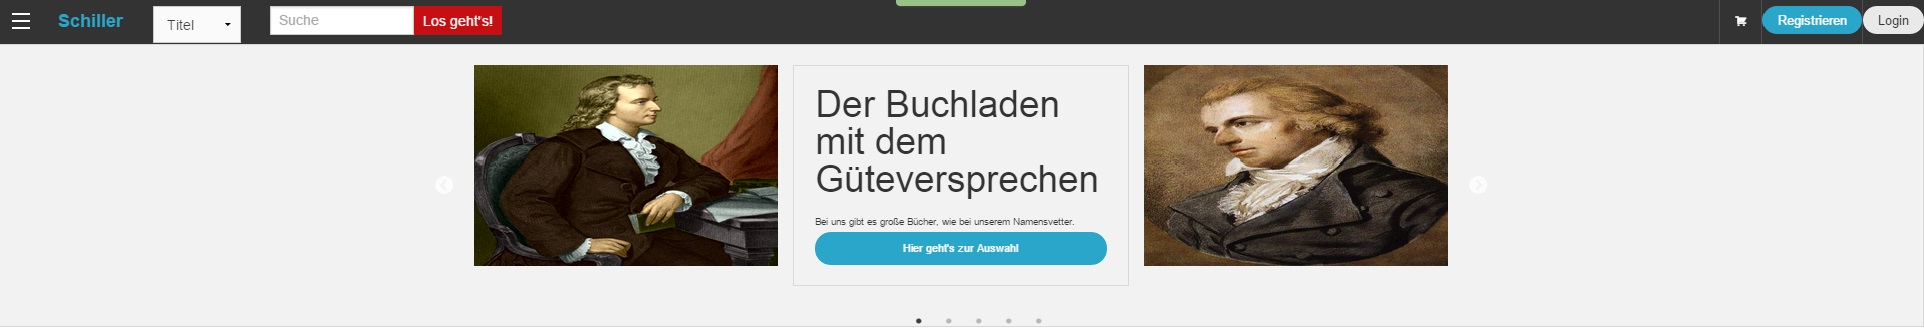
\includegraphics[width=1.0\textwidth]{Topbar1.jpg}
\caption{Topbar und Slider für uneingeloggte Nutzer}	
\end{figure}
\smallskip

\begin{figure}[ht]
\centering
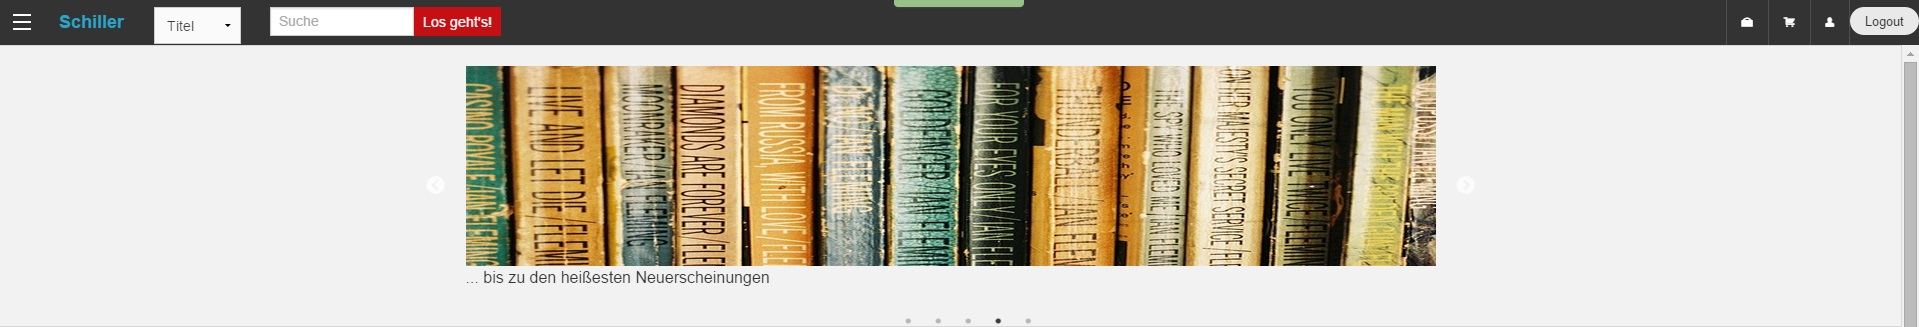
\includegraphics[width=1.0\textwidth]{Topbar2.jpg}
\caption{Topbar und Slider für eingeloggte Kunden}
\end{figure}
\smallskip

\begin{figure}[ht]
\centering
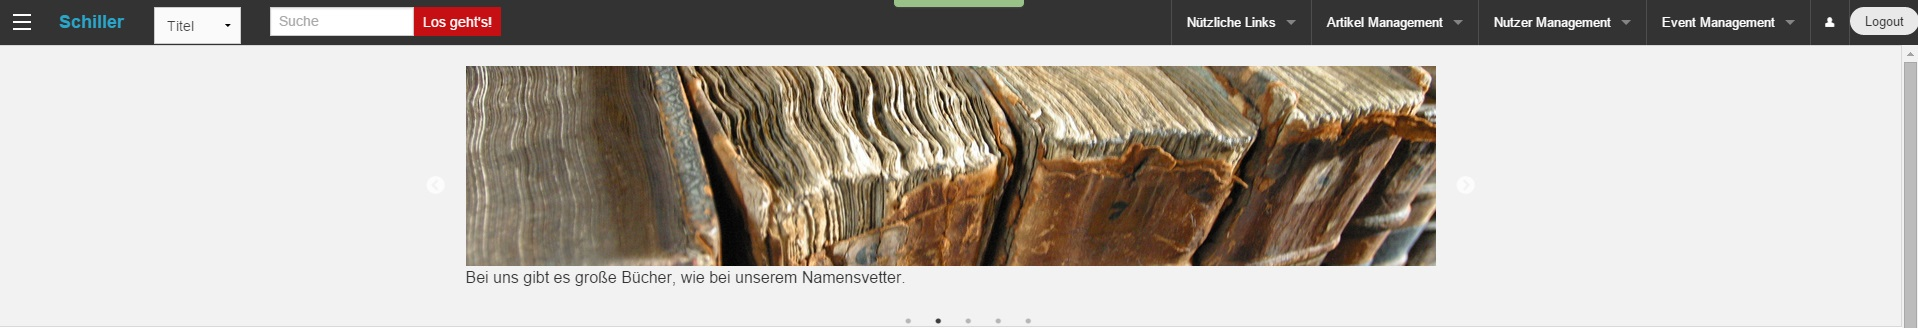
\includegraphics[width=1.0\textwidth]{Topbar3.jpg}
\caption{Topbar und Slider für einen eingeloggten Admin}
\end{figure}
\smallskip

\begin{figure}[ht]
\centering
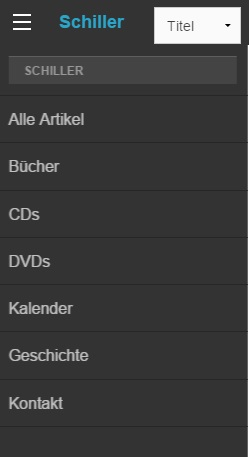
\includegraphics[width=0.2\textwidth]{Sidebar.jpg}
\caption{Sidebar}
\end{figure}
\smallskip

\FloatBarrier

\subsection{Startseite} \label{startseite} 

Auf der Startseite finden Sie eine Übersicht über verschiedene Artikel (inkl. Titel, Künstler, Coverbild und Preis) der Buchhandlung Schiller. Hierbei wird ein Artikel besonders groß dargestellt (inkl. Titel, Künstler, Coverbild, Preis und Artikelbeschreibung). Die Artikel kann man durch Klicken auf den entsprechenden Button zum Warenkorb hinzufügen. \\

\begin{figure}[ht]
\centering
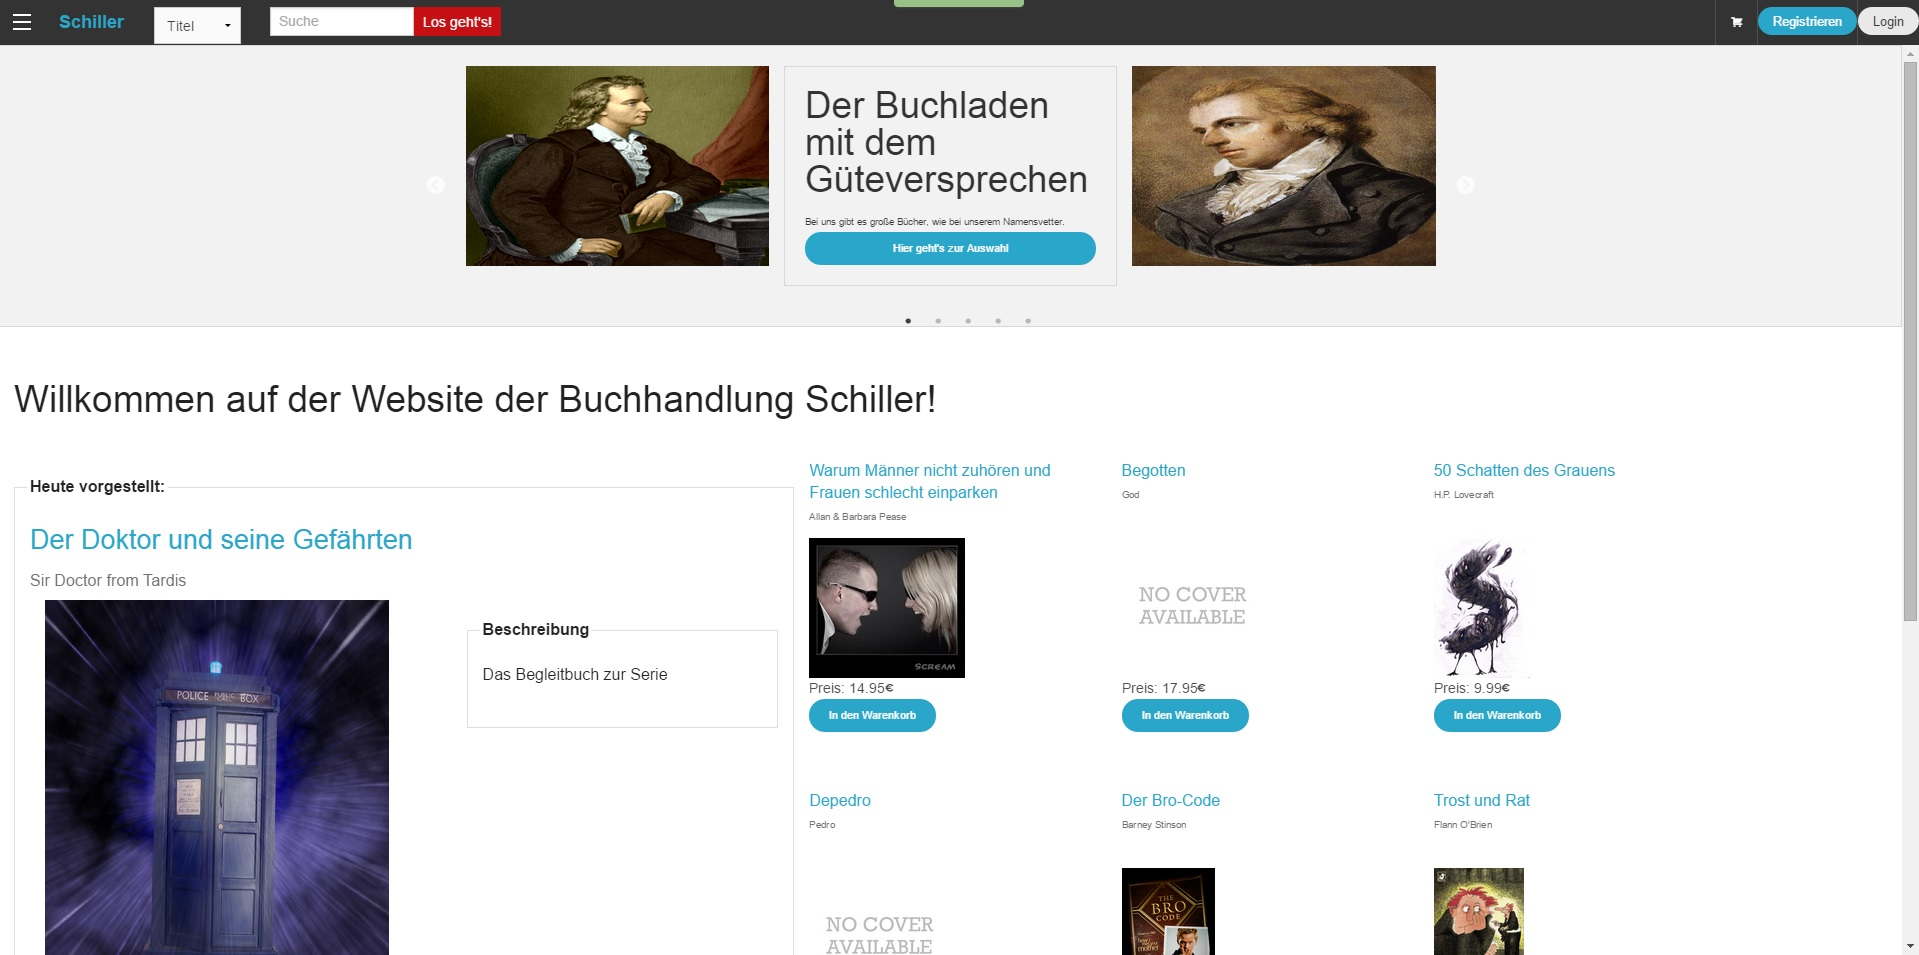
\includegraphics[width=1.0\textwidth]{Startseite.jpg}
\caption{Startseite}
\end{figure}
\smallskip

\FloatBarrier

\subsection{Registrierung}

Nicht eingeloggte Nutzer gelangen durch klicken auf den Link ''Registrieren'' in der Topbar zum Registrierungsformular. \\
Hier müssen verschiedene personenbezogene Daten (Vorname, Nachname, Straße, Nummer, PLZ, Ort) und Accountdaten (Nutzername, E-Mail, Passwort, Passwortwiederholung) angegeben werden. Ist das Format der eingegebenen Daten nicht korrekt, dann erscheinen direkt nach Eingabe Fehlermeldungen und die Registrierung ist nicht möglich. Sind Nutzername bzw. E-Mail bereits vergeben, so erscheinen direkt nach Klicken auf den Button ''Registrieren'' Fehlermeldungen und es findet keine Registrierung statt. Nur wenn alle eingegebenen Daten syntaktisch korrekt sind, wird der Nutzer mit den angegebenen Daten als Kunde registriert.

\begin{figure}[ht]
\centering
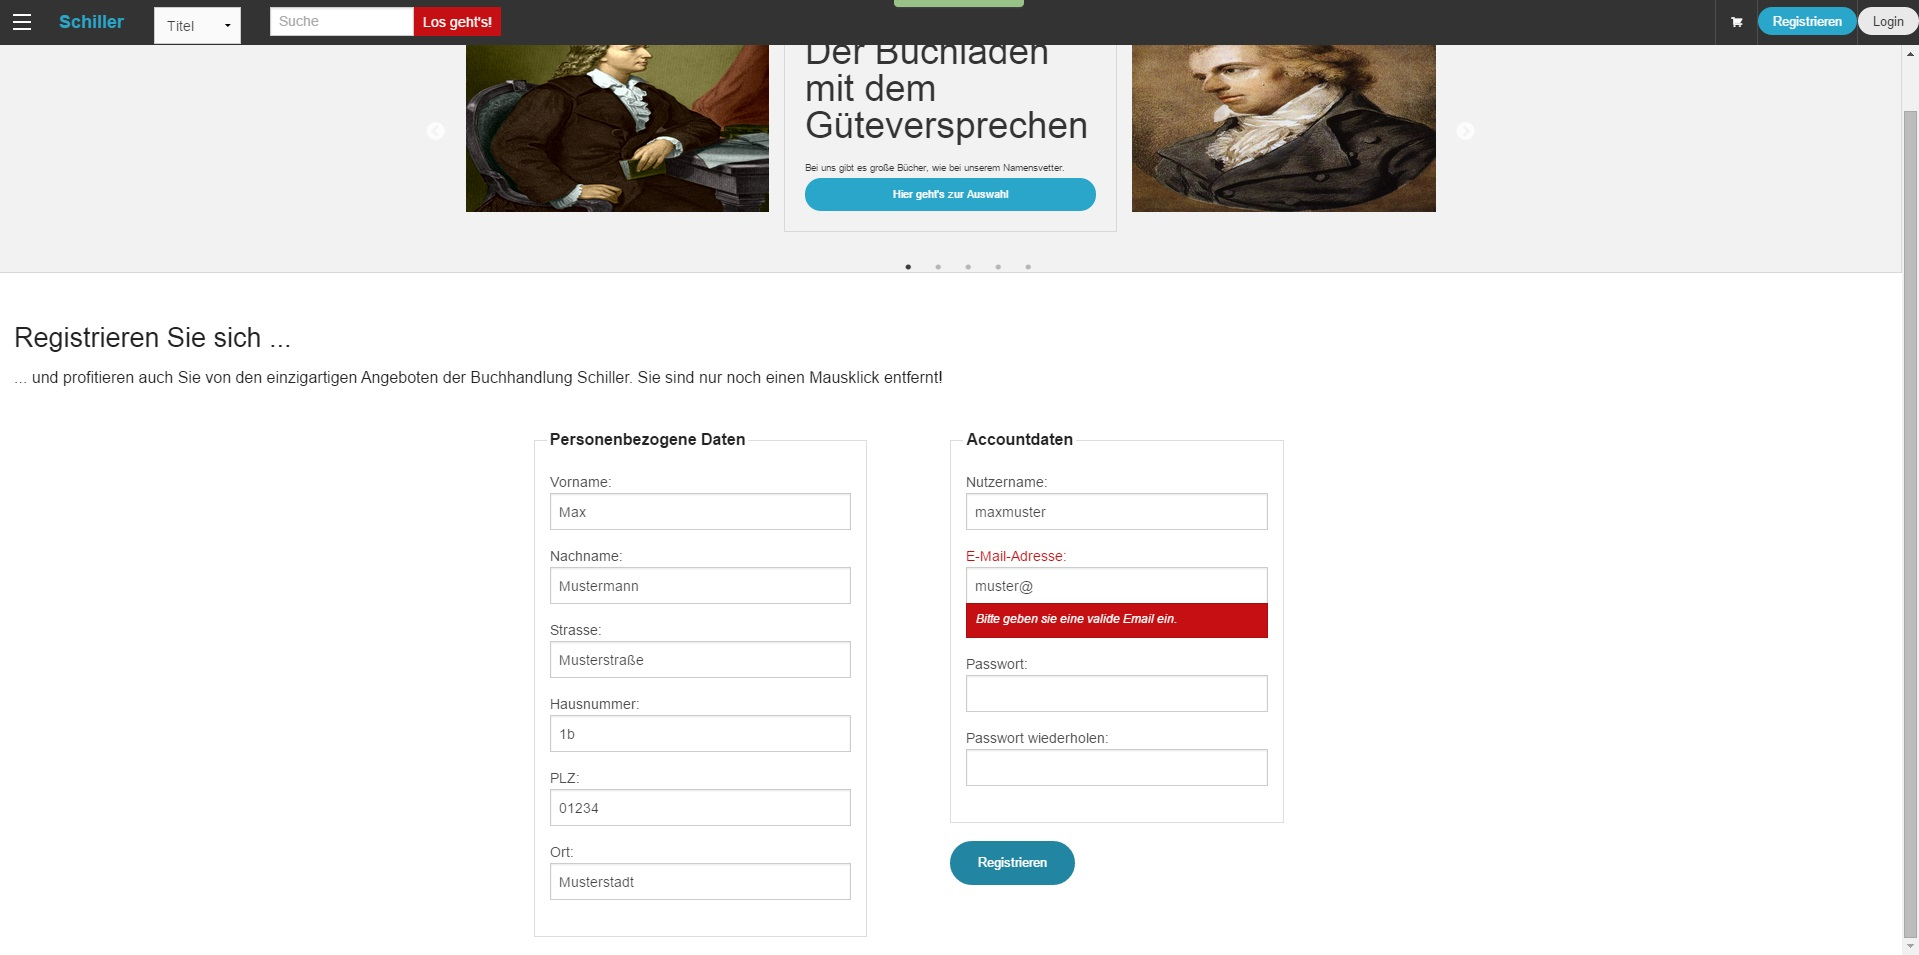
\includegraphics[width=1.0\textwidth]{Registrierung.jpg}
\caption{Registrierungsformular}
\end{figure}
\smallskip

\FloatBarrier

\subsection{Login}

Um auf alle verfügbaren Funktionen der Buchhandlung Schiller zugreifen zu können, muss der Nutzer sich zunächst anmelden. \\
Nicht eingeloggte Nutzer gelangen durch Klicken auf den Link ''Login'' in der Topbar zur Login-Seite der Anwendung. Hier müssen nun Benutzername und Passwort des Nutzers eingegeben werden. Ist der Benutzername nicht vorhanden oder das zugehörige Passwort nicht korrekt, dann ist eine Anmeldung im System nicht möglich und die Daten müssen erneut eingegeben werden. Sind alle eingegeben Daten korrekt, so wird der Nutzer in das System eingeloggt.

\begin{figure}[ht]
\centering
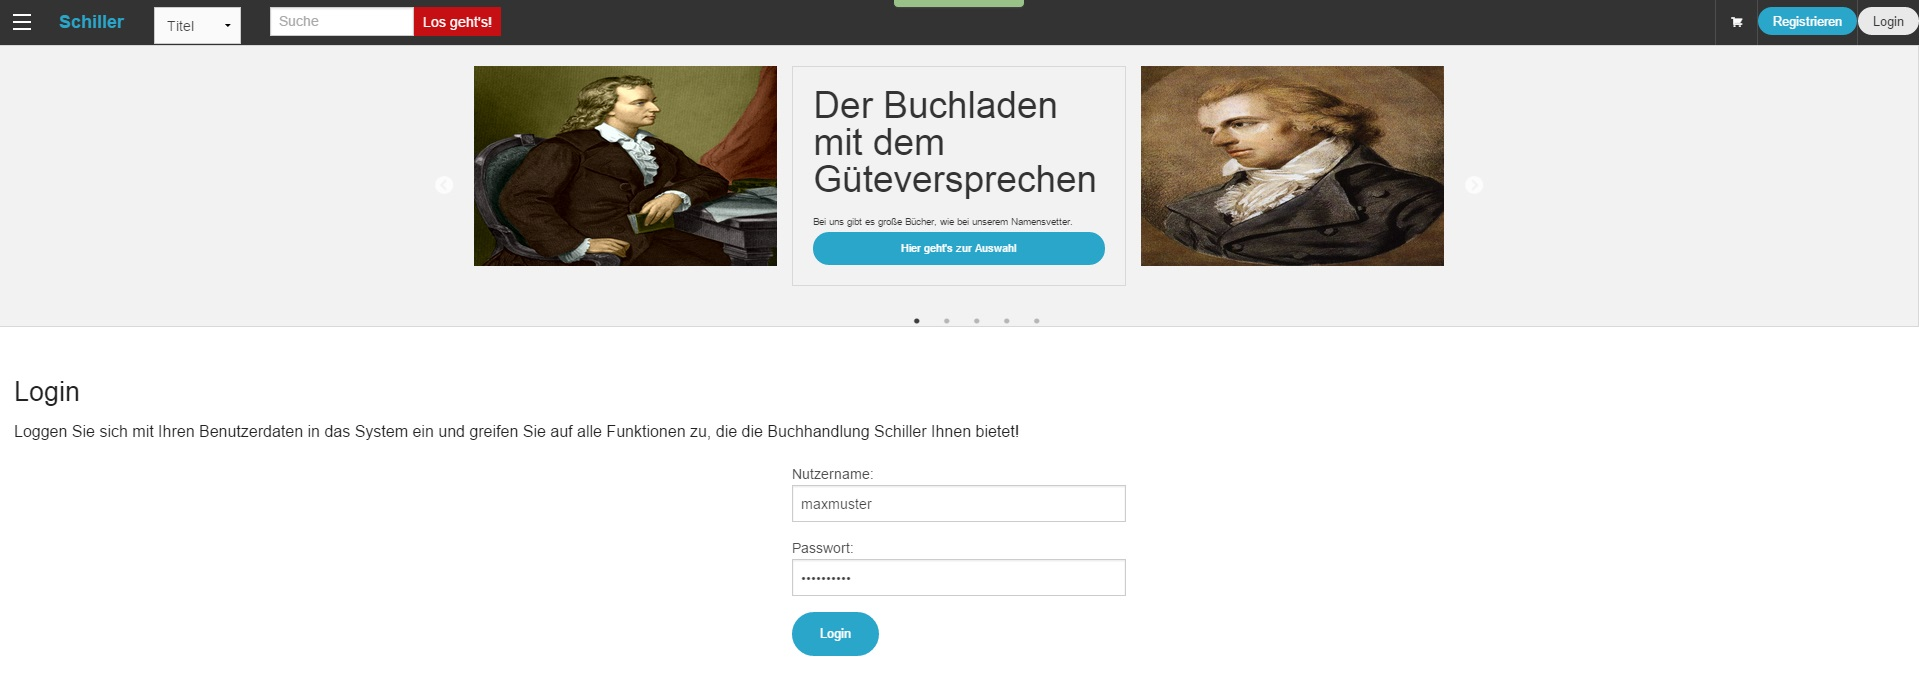
\includegraphics[width=1.0\textwidth]{Login.jpg}
\caption{Login-Seite}
\end{figure}
\smallskip

\FloatBarrier

\subsection{Logout}

Eingeloggte Nutzer können sich durch Klicken auf den Button ''Logout'' in der Topbar aus dem System ausloggen.

\newpage

\section{Allgemeine Funktionen}

\subsection{Eigene Profilansicht und -bearbeitung} \label{profil}

Eingeloggte Nutzer gelangen durch Klicken auf das Torso-Symbol in der Topbar zur eigenen Profilansicht. \\
Hier werden Nutzername, Name, Adresse, E-Mail und ein Standard-Profilbild des eigenen Accounts aufgeführt. Nutzern mit den Rollen ''Admin'', ''Boss'' oder ''Usermanager'' werden zusätzlich Rollen und Status (aktiviert oder deaktiviert) des eigenen Accounts angezeigt. \\
Zur Änderungsansicht der eigenen Profildaten kann der Nutzer durch Klicken auf den entsprechenden Link über den Profildaten gelangen. Hier sind die aktuellen Daten des eigenen Nutzeraccounts schon voreingetragen. Der Nutzer kann diese nun ändern. Hierbei muss er sein korrektes altes Passwort eingeben. Außerdem muss er sein neues Passwort eingeben und dieses wiederholen. Wenn eine Änderung des Passwortes nicht erwünscht ist, so muss das alte Passwort des Nutzers in alle drei Felder eingetragen werden. Ist das Format der eingegebenen Daten nicht korrekt, dann erscheinen direkt nach der Eingabe Fehlermeldungen und die Profiländerung ist nicht möglich. Ist die E-Mail bereits vergeben, das alte Passort falsch oder das neue Passwort falsch wiederholt, so erscheinen direkt nach Klicken auf den Button ''Neue Profildaten speichern'' Fehlermeldungen und es findet keine Profiländerung statt. Nur wenn alle eingegebenen Daten syntaktisch korrekt sind, werden die Profildaten des Nutzers entsprechend geändert und der Nutzer wird zur eigenen Profilansicht weitergeleitet.

\begin{figure}[ht]
\centering
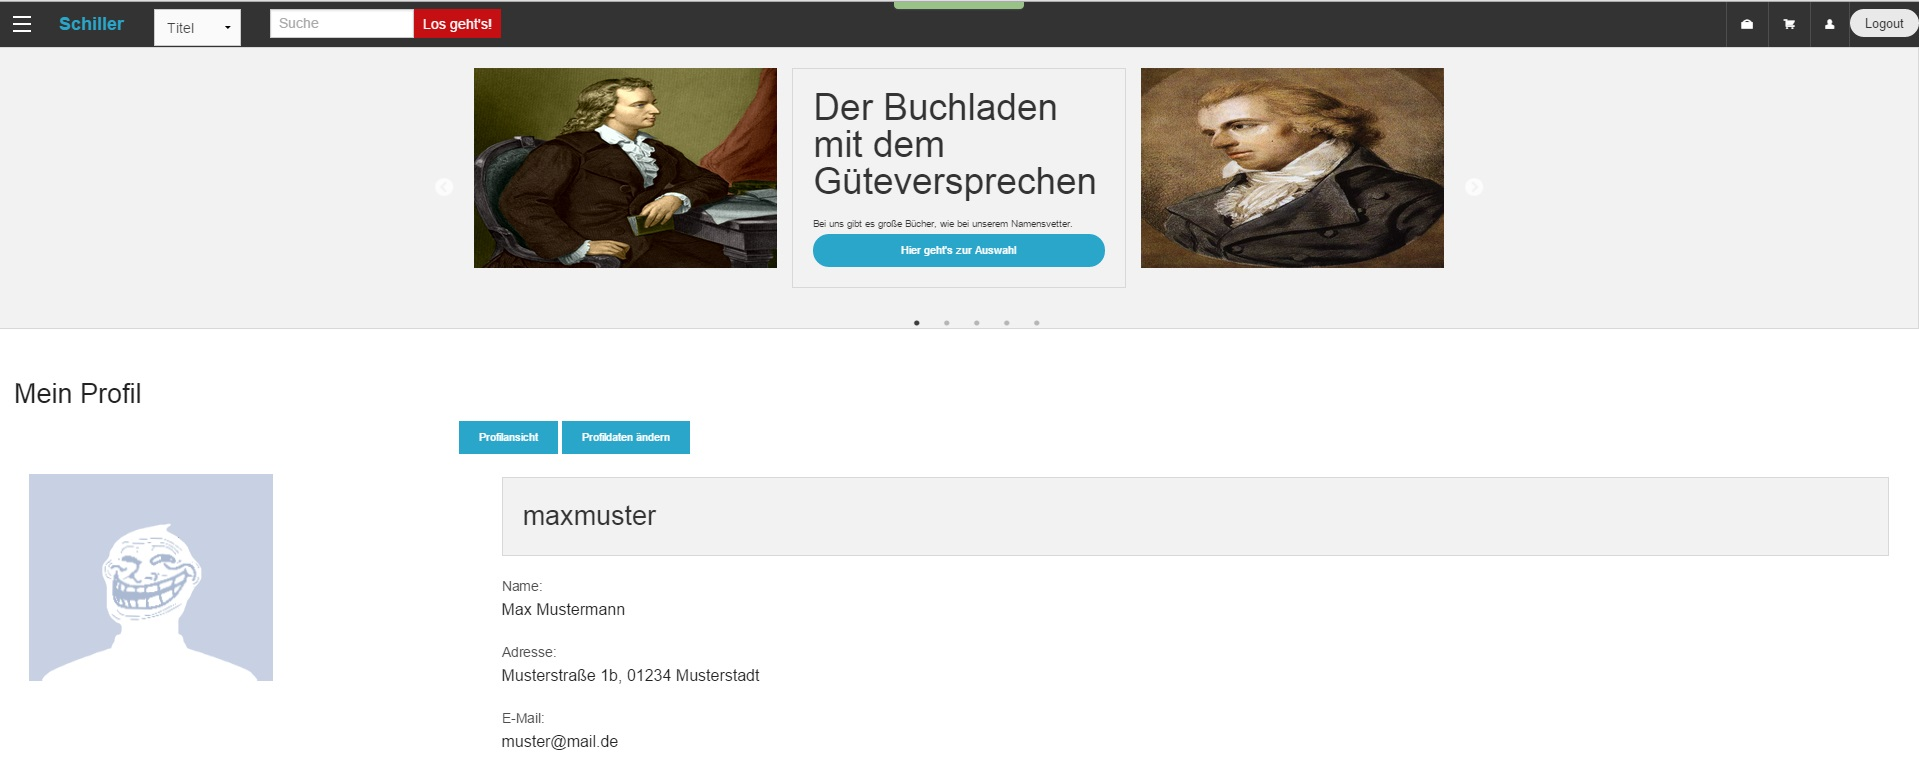
\includegraphics[width=1.0\textwidth]{Profil.jpg}
\caption{Eigene Profilansicht}
\end{figure}
\smallskip

\begin{figure}[ht]
\centering
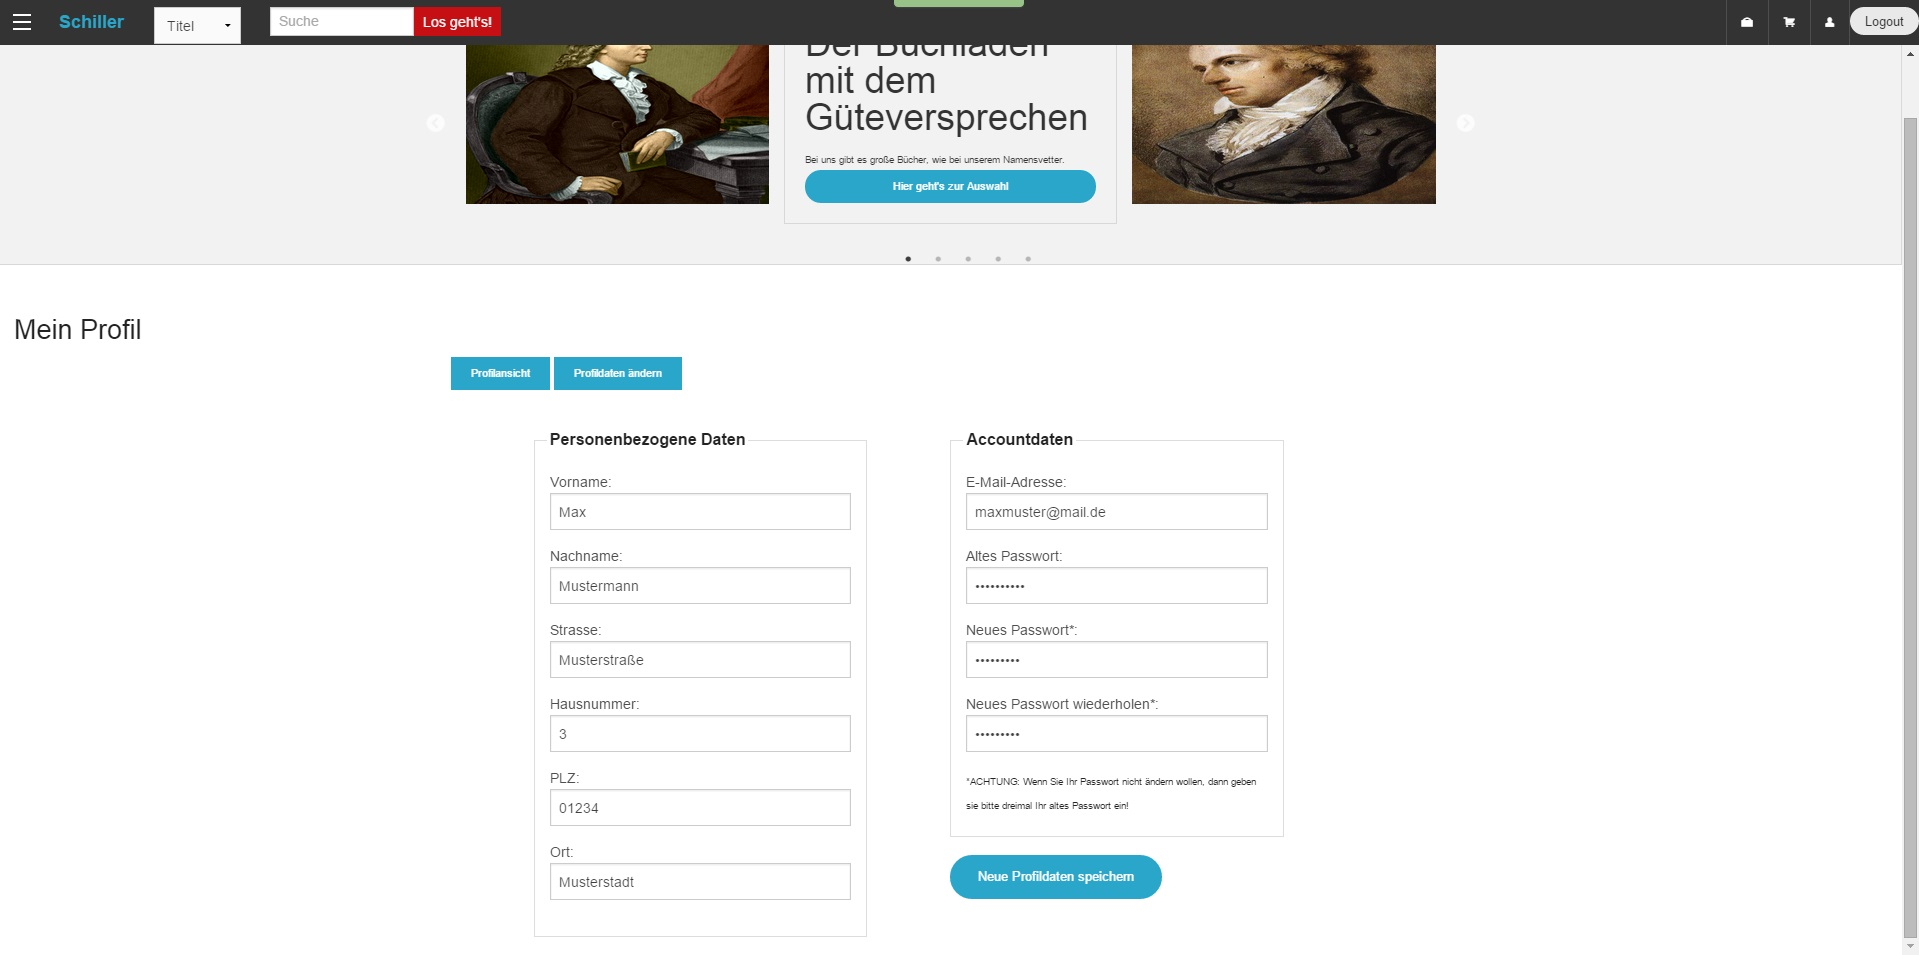
\includegraphics[width=1.0\textwidth]{Profilaenderung.jpg}
\caption{Profiländerung des eigenen Profils}
\end{figure}
\smallskip

\FloatBarrier

\subsection{Artikelübersicht} \label{ansicht} 

Alle Nutzer (egal ob eingeloggt oder nicht) können in der linken Sidebar bestimmte Artikelansichten auswählen. \\
Durch Klicken auf ''Alle Artikel'' gelangt man zu einer Ansicht mit allen verfügbaren Artikeln (inkl. Titel, Künstler, Coverbild und Preis). Durch Klicken auf ''Bücher'', ''CD's'' oder ''DVD's'' gelangt man zu einer Ansicht, wo jeweils alle verfügbaren Bücher, CD's bzw. DVD's (inkl. Titel, Künstler, Coverbild und Preis) aufgeführt sind. Auf jeder dieser Ansichtsseiten kann eine bestimmte Anzahl des Artikels durch Klicken auf den entsprechenden Button zum Warenkorb hinzugefügt werden.

\begin{figure}[ht]
\centering
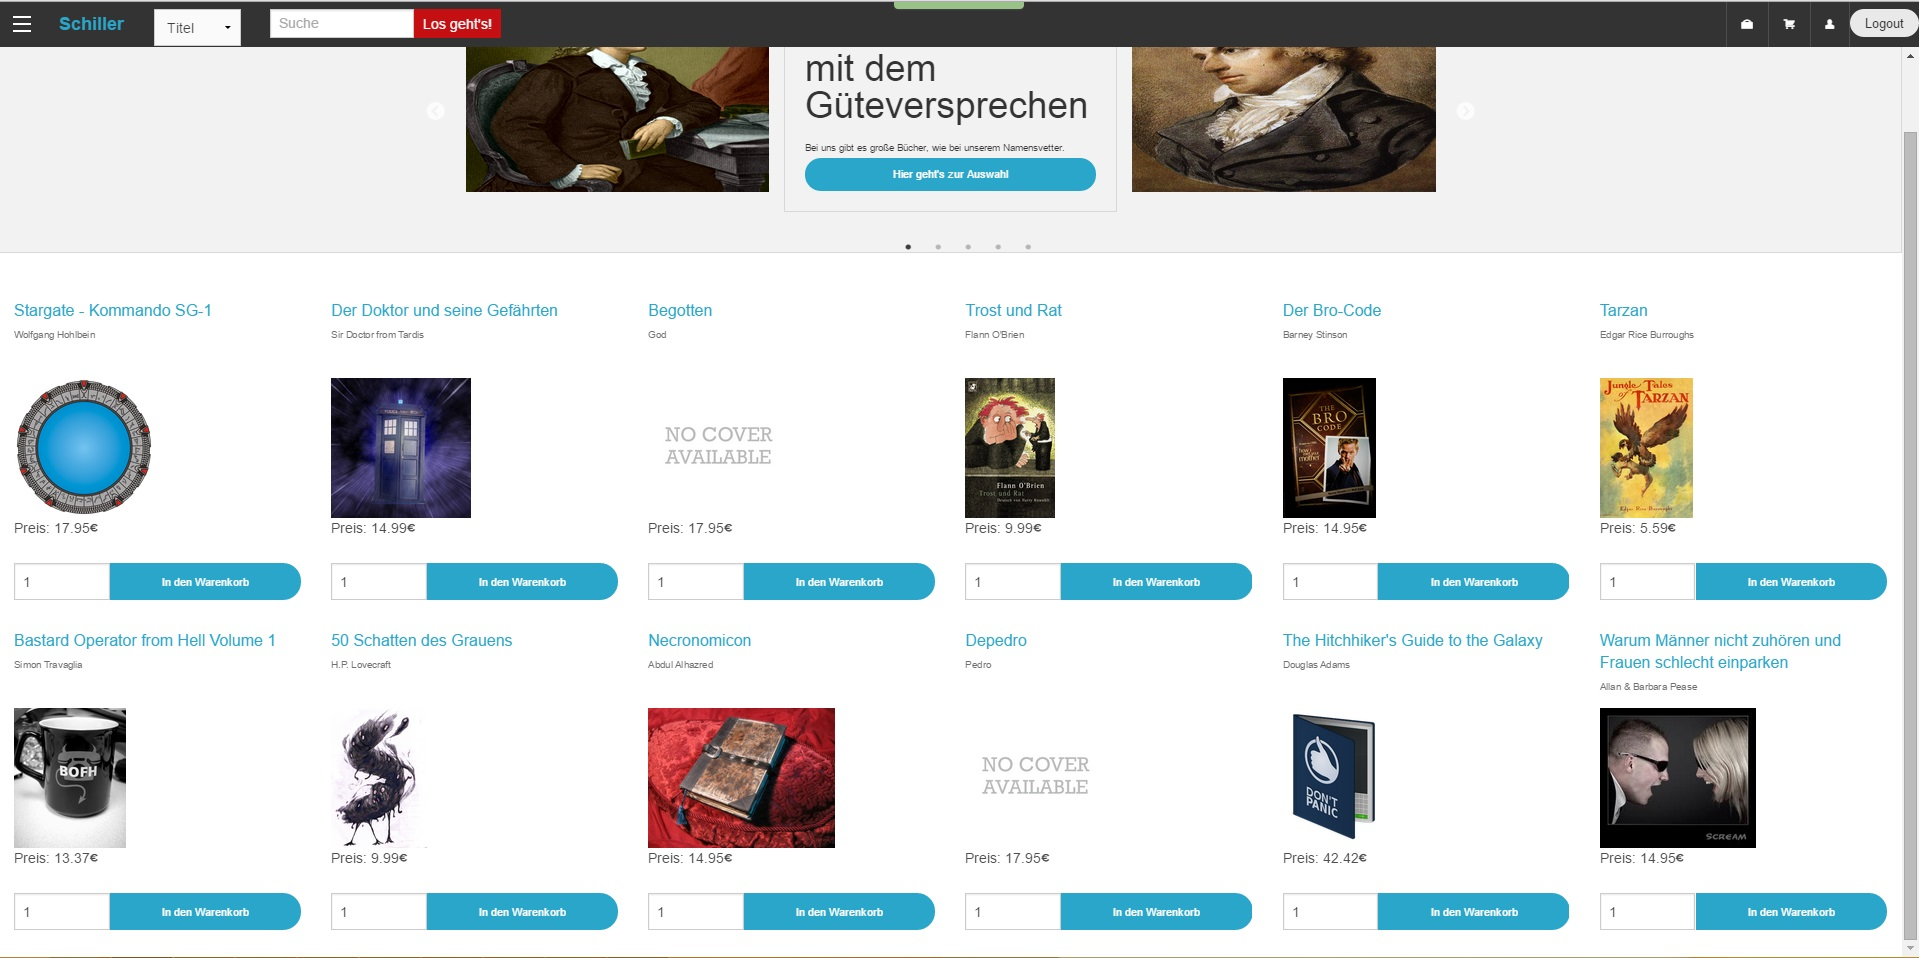
\includegraphics[width=1.0\textwidth]{Artikel.jpg}
\caption{Übersicht über alle Artikel}
\end{figure}
\smallskip

\FloatBarrier

\subsection{Suche nach bestimmten Artikeln} \label{suche} 

Alle Nutzer (egal ob eingeloggt oder nicht) können mithilfe des Suchfeldes in der Topbar nach bestimmten Artikeln suchen. Dazu muss zunächst in der Dropdown-Liste links neben dem Suchfeld ausgewählt werden, ob die Artikel nach Titel, Verlag, ISBN, Künstler oder Kategorie gefiltert werden sollen. Ich Suchfeld kann man nun eine beliebige Folge von Zeichen eingeben. \\
Durch Klicken auf den Link ''Los geht's'' wird man auf eine Ansichtsseite weitergeleitet mit allen Artikeln (inkl. Titel, Künstler, Coverbild und Preis), die die eingegebene Zeichenfolge in der, mithilfe der Dropdown-Liste, ausgewählten Komponente enthalten. Bei Eingabe von drei oder weniger Zeichen werden nur die Artikel angezeigt, bei denen die Zeichenfolge am Anfang der ausgewählten Komponente steht. Auf dieser Ansichtsseite kann eine bestimmte Anzahl des Artikels durch Klicken auf den entsprechenden Button zum Warenkorb hinzugefügt werden.

\begin{figure}[ht]
\centering
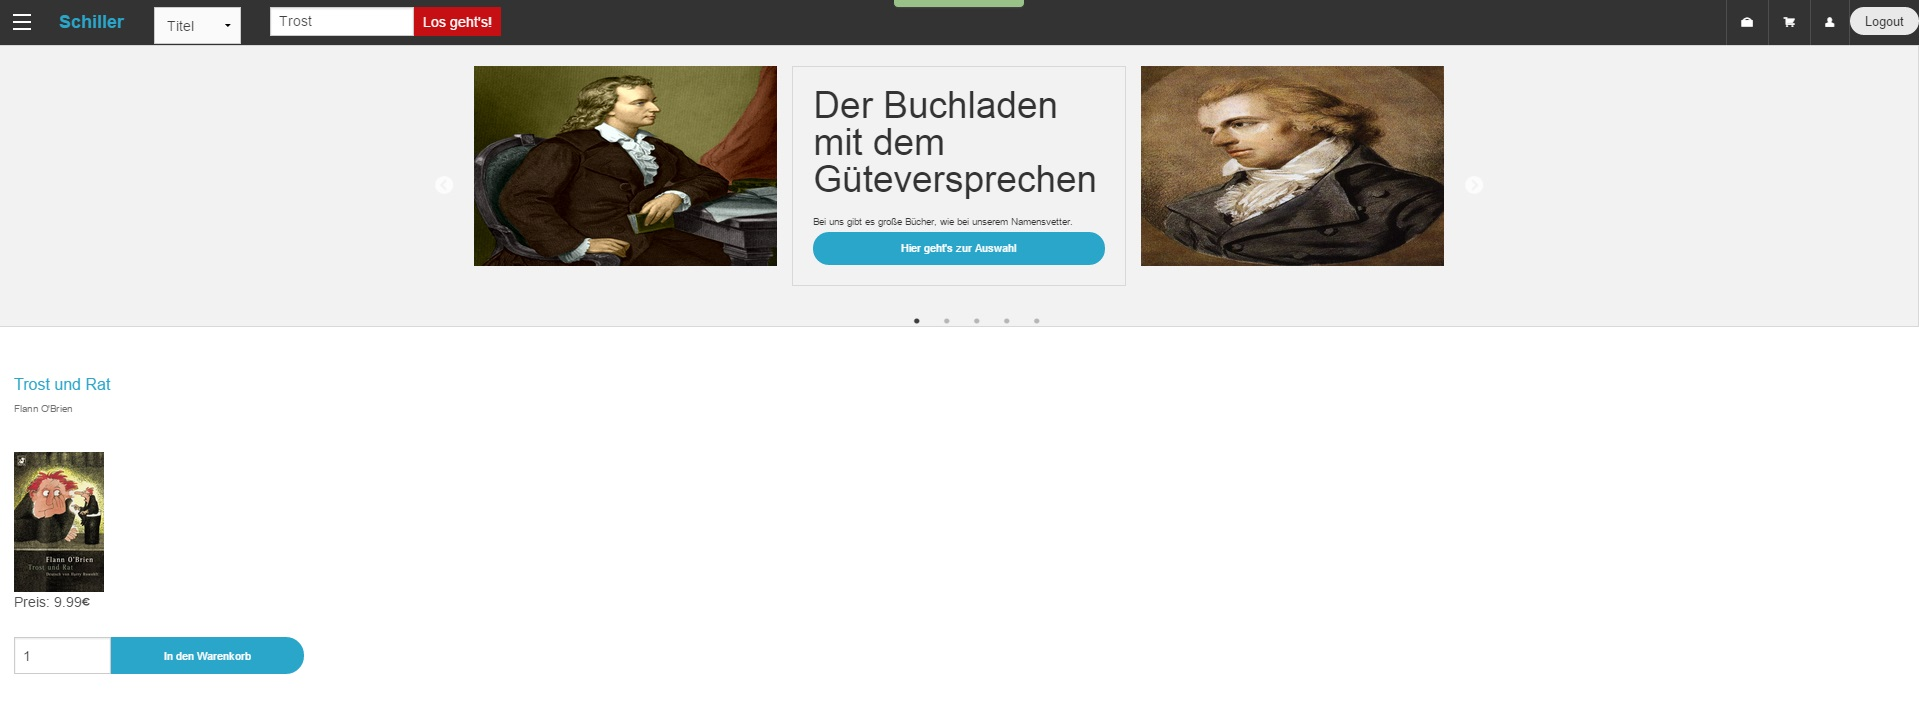
\includegraphics[width=1.0\textwidth]{Suche.jpg}
\caption{Suche nach dem Schlagwort ''Trost''}
\end{figure}
\smallskip

\FloatBarrier

\subsection{Detailansicht eines einzelnen Artikels} \label{detail}

Alle Nutzer (egal ob eingeloggt oder nicht) können von jeder Ansichtseite mehrerer Artikel (entsprechend \ref{startseite}, \ref{ansicht} bzw. \ref{suche}) durch Klicken auf den jeweiligen Titel auf die Detailansicht des Artikels zugreifen. \\
Hier werden Titel, Künstler, Artikelnummer (entspricht bei Büchern der ISBN), aktueller Lagerbestand, Verlag, Kategorien, Preis, Coverbild und Artikelbeschreibung aufgeführt. Außerdem lässt sich eine bestimmte Anzahl des Artikels durch Klicken auf den entsprechenden Button zum Warenkorb hinzufügen. \\
Nutzer mit bestimmten Rollen können auf dieser Seite noch weitere Aktionen ausführen (siehe dazu \ref{artikeländerung}).

\begin{figure}[ht]
\centering
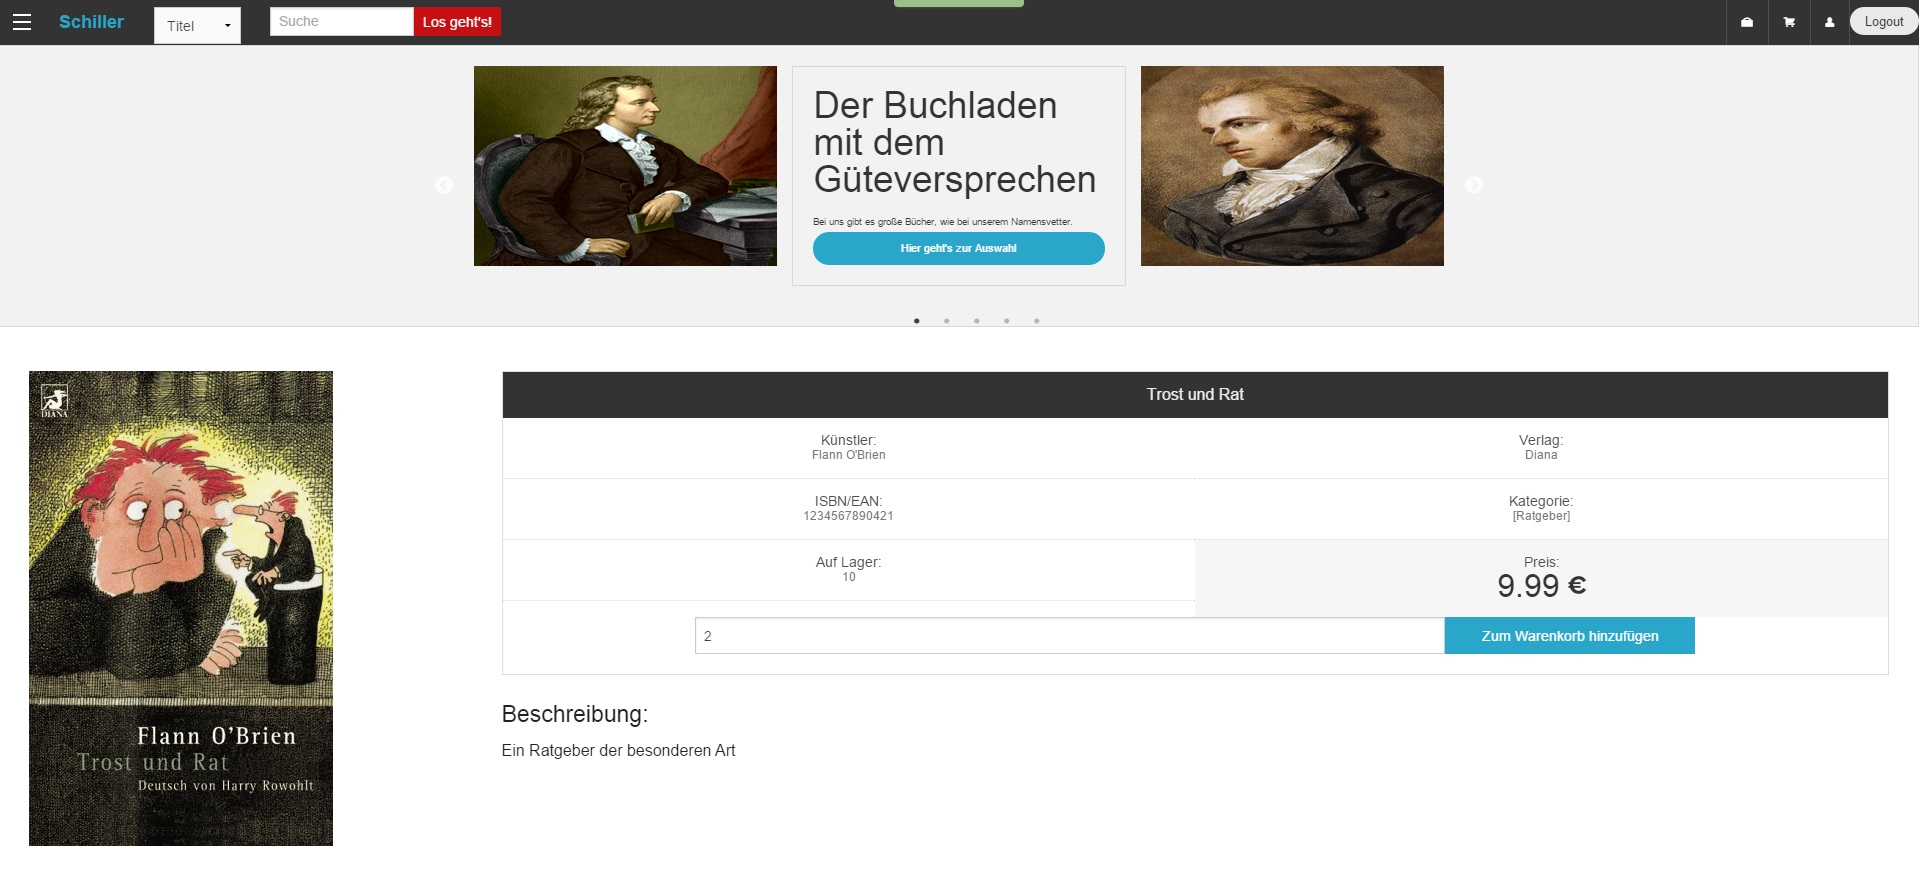
\includegraphics[width=1.0\textwidth]{Artikeldetail.jpg}
\caption{Detailansicht eines Artikels}
\end{figure}
\smallskip

\FloatBarrier

\subsection{Eigene Warenkorbansicht}

Alle Kunden und nicht eingeloggten Nutzer gelangen durch Klicken auf das Warenkorb-Symbol in der Topbar zur eigenen Warenkorbansicht. \\
Hier werden in einer Liste alle im Warenkorb liegenden Artikel (inkl. Titel, Anzahl und Preis) angegeben. Unter der Liste ist der Gesamtpreis der Warenkorbs aufgeführt. Mithilfe der Buttons ''Löschen'' kann der Nutzer einzelne Artikel aus dem Warenkorb entfernen. Mithilfe des Buttons ''Leeren'' kann der Nutzer alle Artikel aus dem Warenkorb entfernen. Ist der Nutzer ein eingeloggter Kunde, so kann er mithilfe des Buttons ''Kaufen'' verbindlich den kompletten Warenkorbinhalt bestellten und wird zur Startseite weitergeleitet. 

\begin{figure}[ht]
\centering
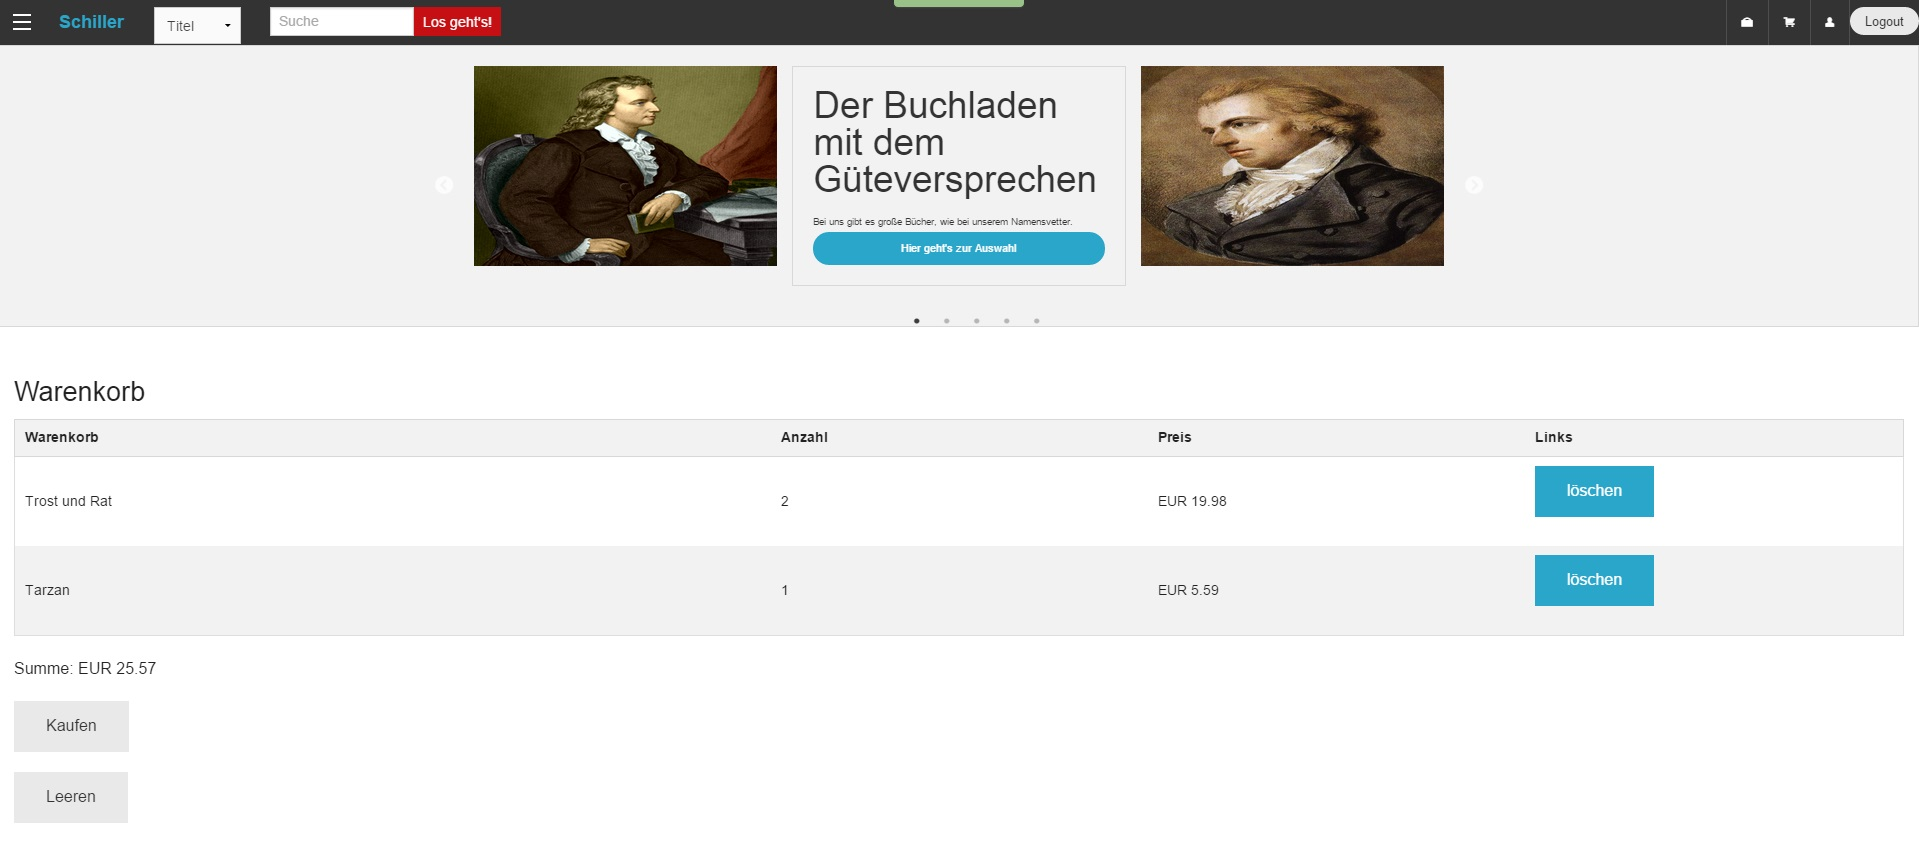
\includegraphics[width=1.0\textwidth]{Warenkorb.jpg}
\caption{Warenkorbansicht}
\end{figure}
\smallskip

\FloatBarrier

\subsection{Kalender- und Reservierungsansicht}

Alle Nutzer (egal ob eingeloggt oder nicht) gelangen durch Klicken auf den Link ''Kalender'' in der Sidebar zur Kalenderansicht. \\
Hier sind in einer Liste alle zukünftig stattfindenden Events (inkl. Datum, Zeit, Eventname, Raumnumer, Raumname, Anzahl der Gesamtsitze und Anzahl davon belegter Sitze) angezeigt. Eingeloggte Kunden können zusätzlich durch Klicken des entsprechenden Buttons einen (oder auch mehrere) Sitzplätze für das Event buchen. Ist die Sitzplatzanzahl voll, so ist das Buchen nicht mehr möglich. \\
Nutzern mit den Rollen ''Admin'', ''Boss'' und ''Eventmanager'' werden zusätzlich zu allen zukünftigen Veranstaltungen auch alle vergangenen Veranstaltungen angezeigt. Außerdem wird für diese Nutzer zu jedem Event ein Link ''Reservierungen'' angezeigt. Durch Klicken dieses Links gelangt der Nutzer zur Reservierungsübersicht des Events. Hier wird in einer Liste für jeden gebuchten Sitzplatz der jeweilige Nutzer angezeigt, der diesen Sitzplatz gebucht hat.

\begin{figure}[ht]
\centering
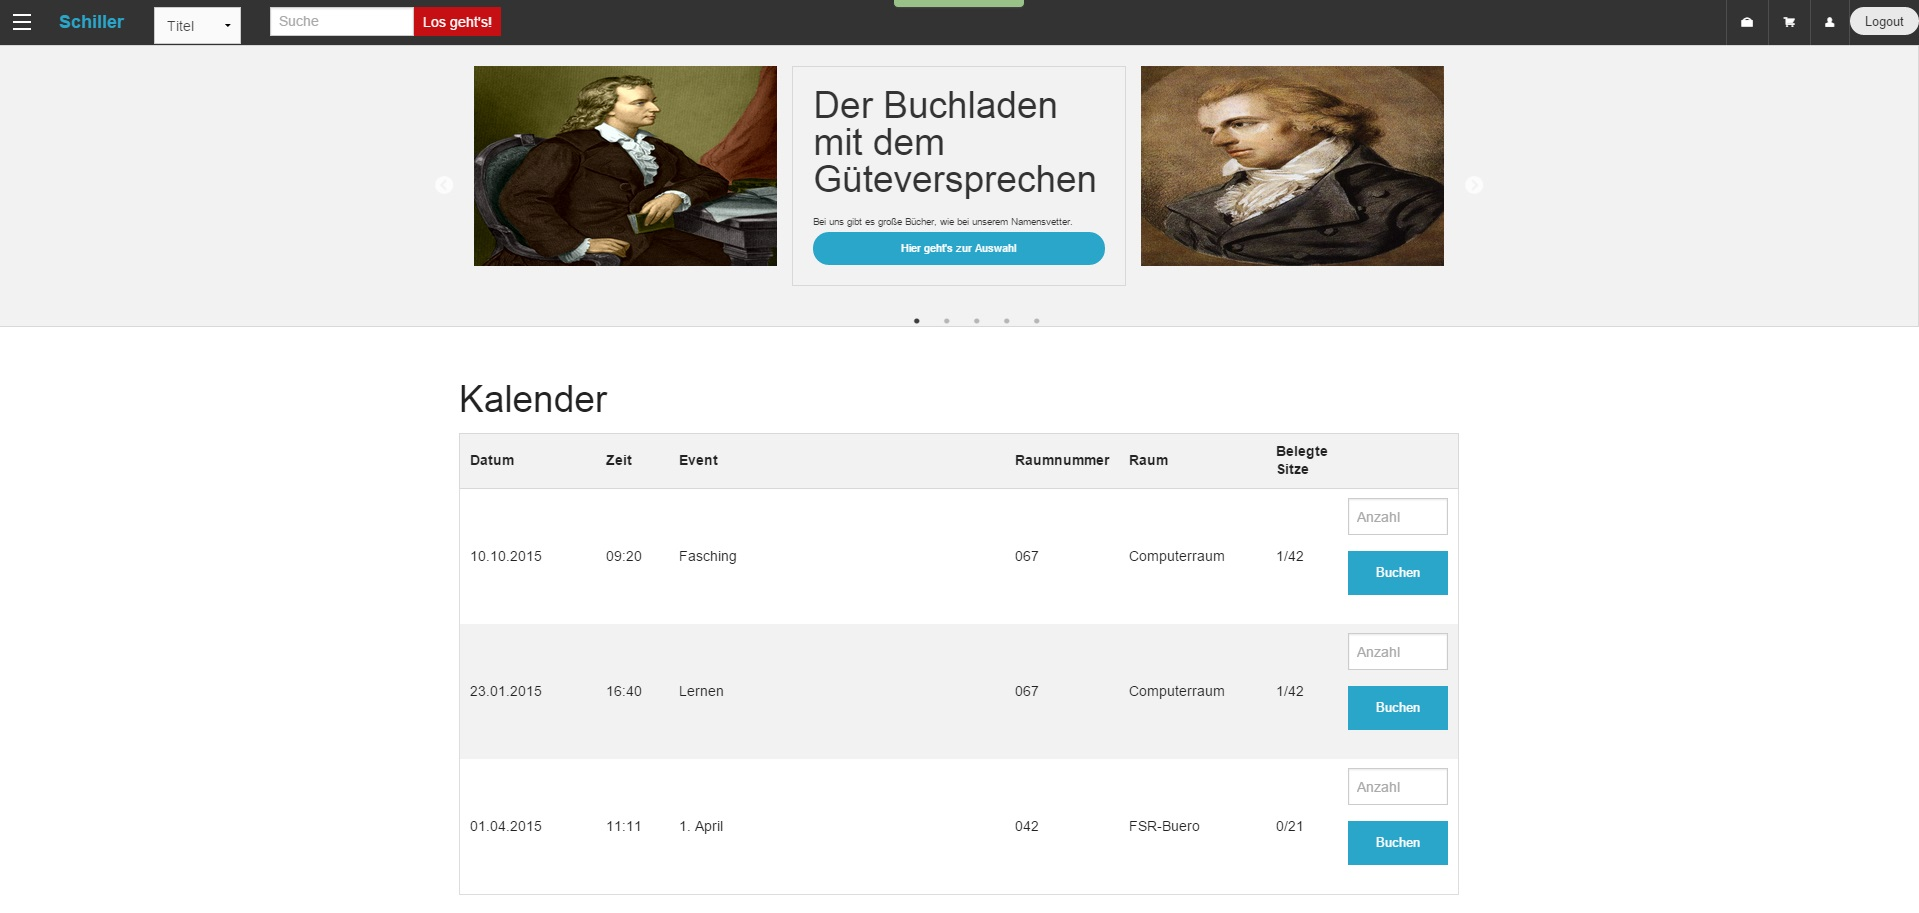
\includegraphics[width=1.0\textwidth]{Kalender1.jpg}
\caption{Kalenderansicht für einen eingeloggten Kunden}
\end{figure}
\smallskip

\begin{figure}[ht]
\centering
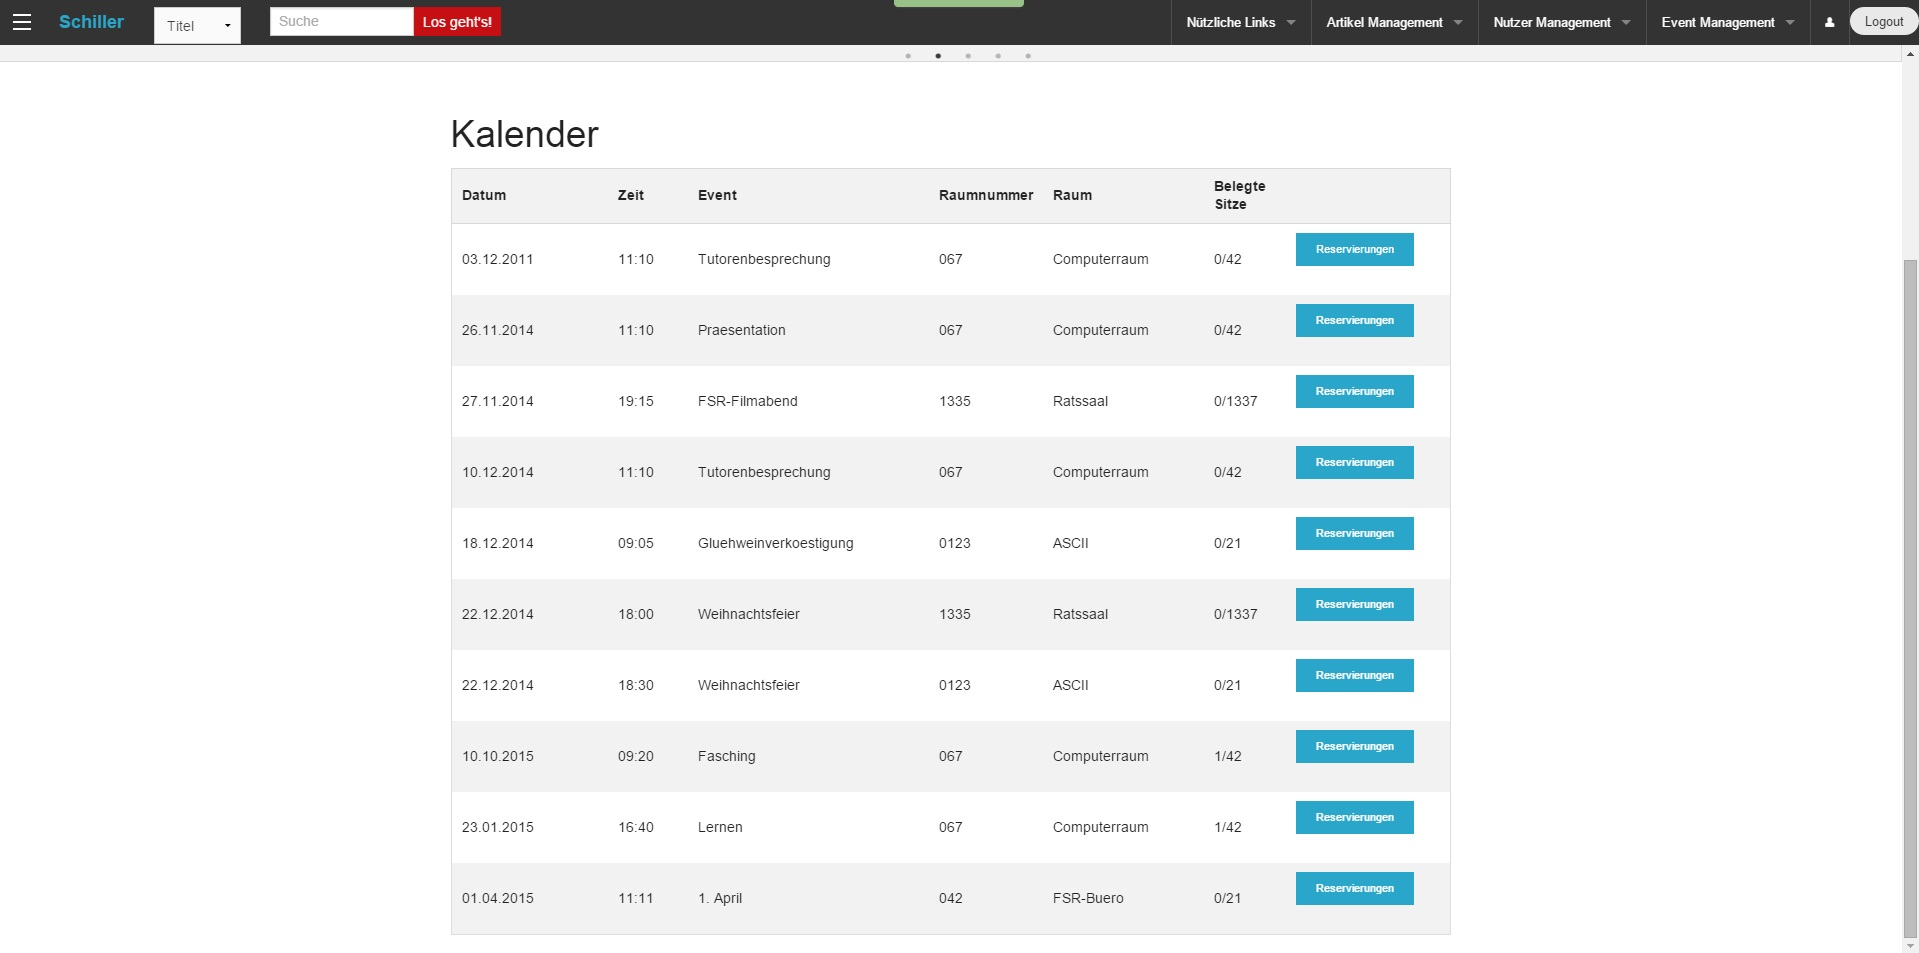
\includegraphics[width=1.0\textwidth]{Kalender2.jpg}
\caption{Kalenderansicht für einen Admin}
\end{figure}
\smallskip

\begin{figure}[ht]
\centering
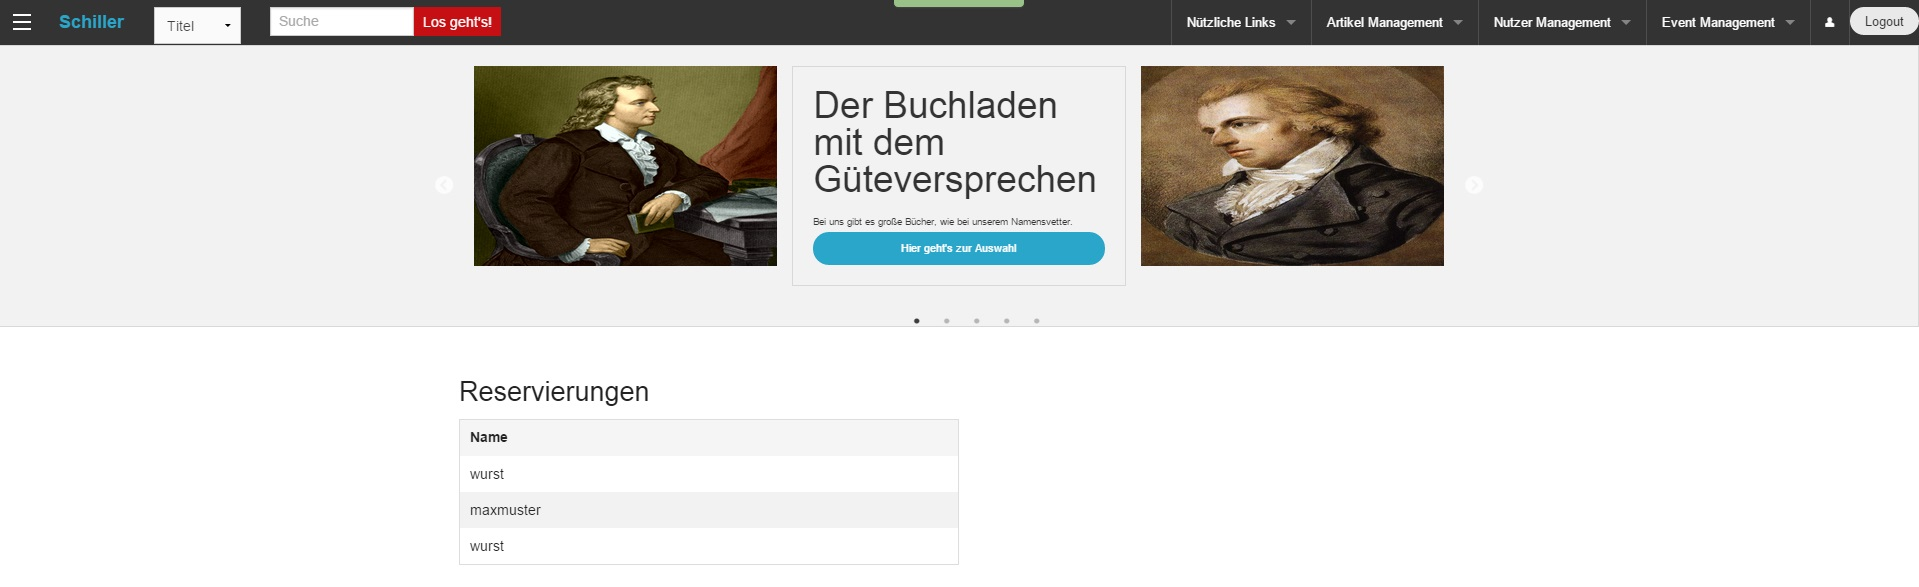
\includegraphics[width=1.0\textwidth]{Kalenderdetail.jpg}
\caption{Detailansicht der Sitzplatzreservierungen für ein Event}
\end{figure}
\smallskip

\FloatBarrier

\subsection{Eigene Bestellungsansicht} \label{bestellung}

Eingeloggte Kunden gelangen durch Klicken auf das Tragetaschen-Symbol in der Topbar zur eigenen Bestellungsansicht. \\
Hier werden in einer Liste alle bisherigen Bestellungen (inkl. Bestellstatus, Zeitstempel und bezahltem Preis) angezeigt. Ist die Bestellung offen (''open''), so kann der Nutzer die Bestellung mithilfe des entsprechenden Buttons stornieren. Sie wird dann sofort als storniert (''cancelled'') angezeigt. Ist die Bestellung bereits durch den zuständigen Angestellten als abgeschlossen (''completed'') markiert worden so ist dies nicht mehr möglich. Für jede Bestellung (egal ob offen, abgeschlossen oder storniert) gelangt der Nutzer über den entsprechenden Link zur Detailansicht der Bestellung. Hier werden alle gekauften Artikel mit ihren jeweiligen Anzahlen angezeigt. Durch Klicken auf den Button Rechnung wird dem Nutzer die PDF-Rechnung inklusive aller Einzel- und Gesamtpreise angezeigt. \\
Außerdem werden in der Bestellübersicht in einer zweiten Tabelle alle bisher getätigten Reservierungen für Events angezeigt. Für jede Reservierung gelangt der Nutzer über den entsprechenden Link zur Detailansicht der Reservierung. Hier werden alle getätigten Reservierungen mit ihren jeweiligen Events, Zeiten und Räumen angezeigt.

\begin{figure}[ht]
\centering
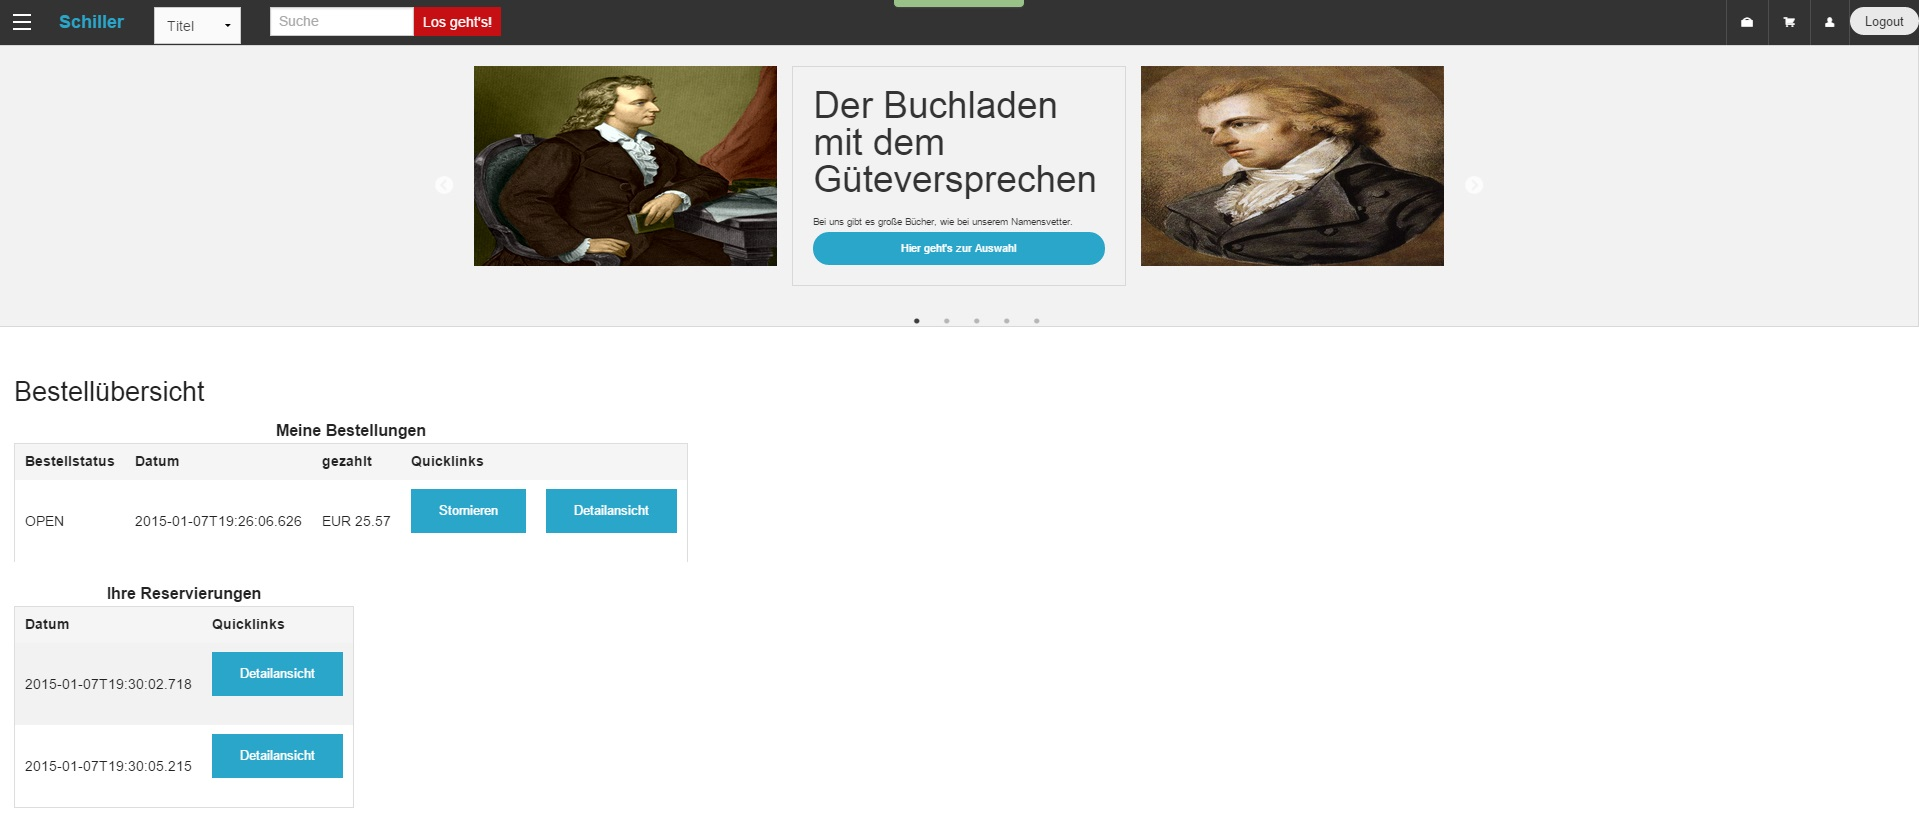
\includegraphics[width=1.0\textwidth]{Bestellungen.jpg}
\caption{Bestellungsübersicht}
\end{figure}
\smallskip

\begin{figure}[ht] 
\centering
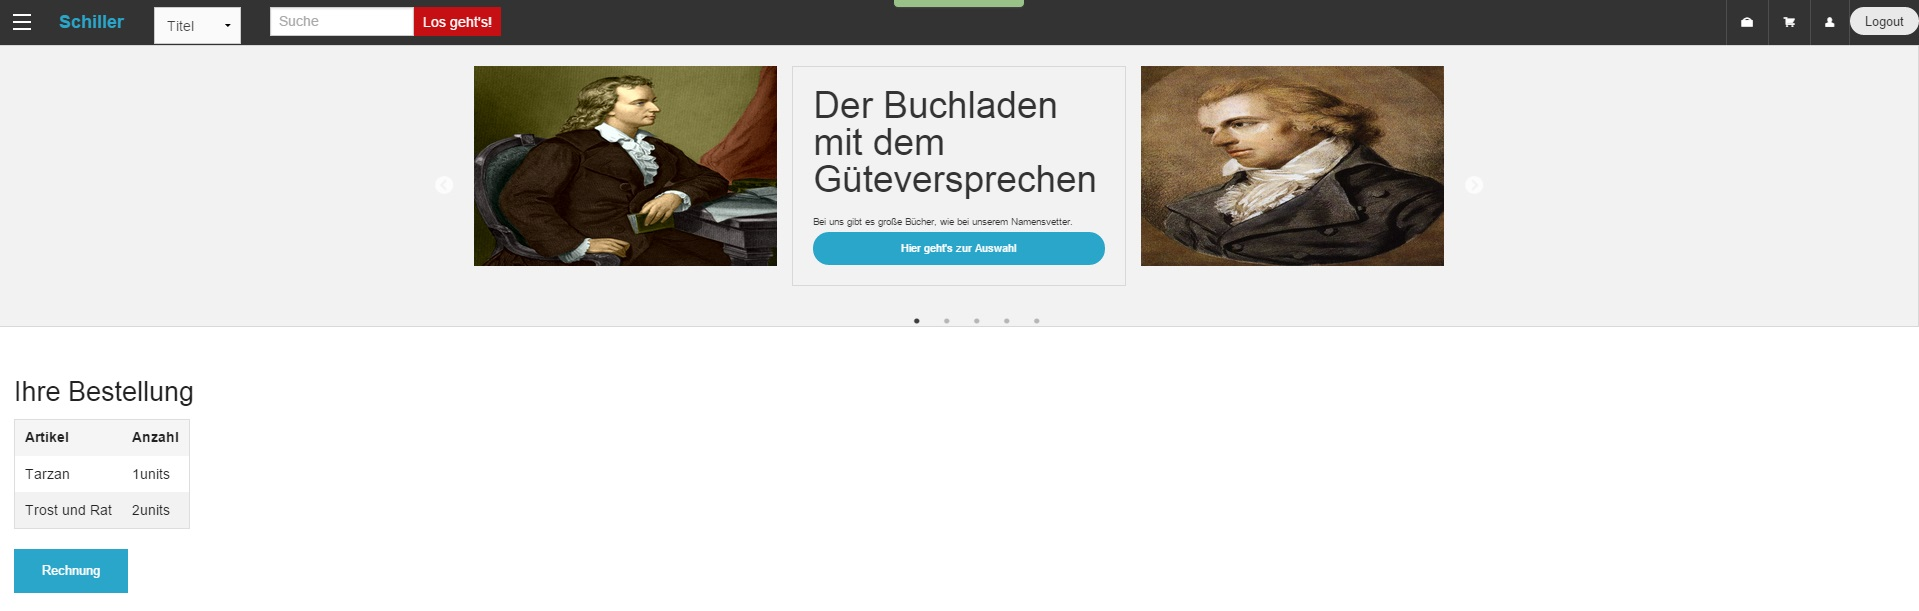
\includegraphics[width=1.0\textwidth]{Bestellungsdetail.jpg}
\caption{Detailansicht einer Bestellung (Reservierung ähnlich)}
\end{figure}
\smallskip

\FloatBarrier

\newpage

\section{Funktionen für spezielle Nutzer}

\subsection{Nutzerübersicht} \label{nutzer}

Nutzer mit den Rollen ''Admin, ''Boss'' und ''Usermanager'' gelangen über die Dropdownliste ''Nutzer Management'' und die Links ''Kundenübersicht'' bzw. ''Angestelltenübersicht'' den entsprechenden Nutzerübersichten. Die Kundenübersicht enthält jeweils Nutzername, Vorname, Nachname, E-Mail-Adresse, Lieferadresse und Status des Kunden. Die Angestelltenübersicht enthält jeweils Nutzername, Vorname, Nachname, Wohnsitz, E-Mail-Adresse, Rollen und Status des Angestellten.

\begin{figure}[ht]
\centering
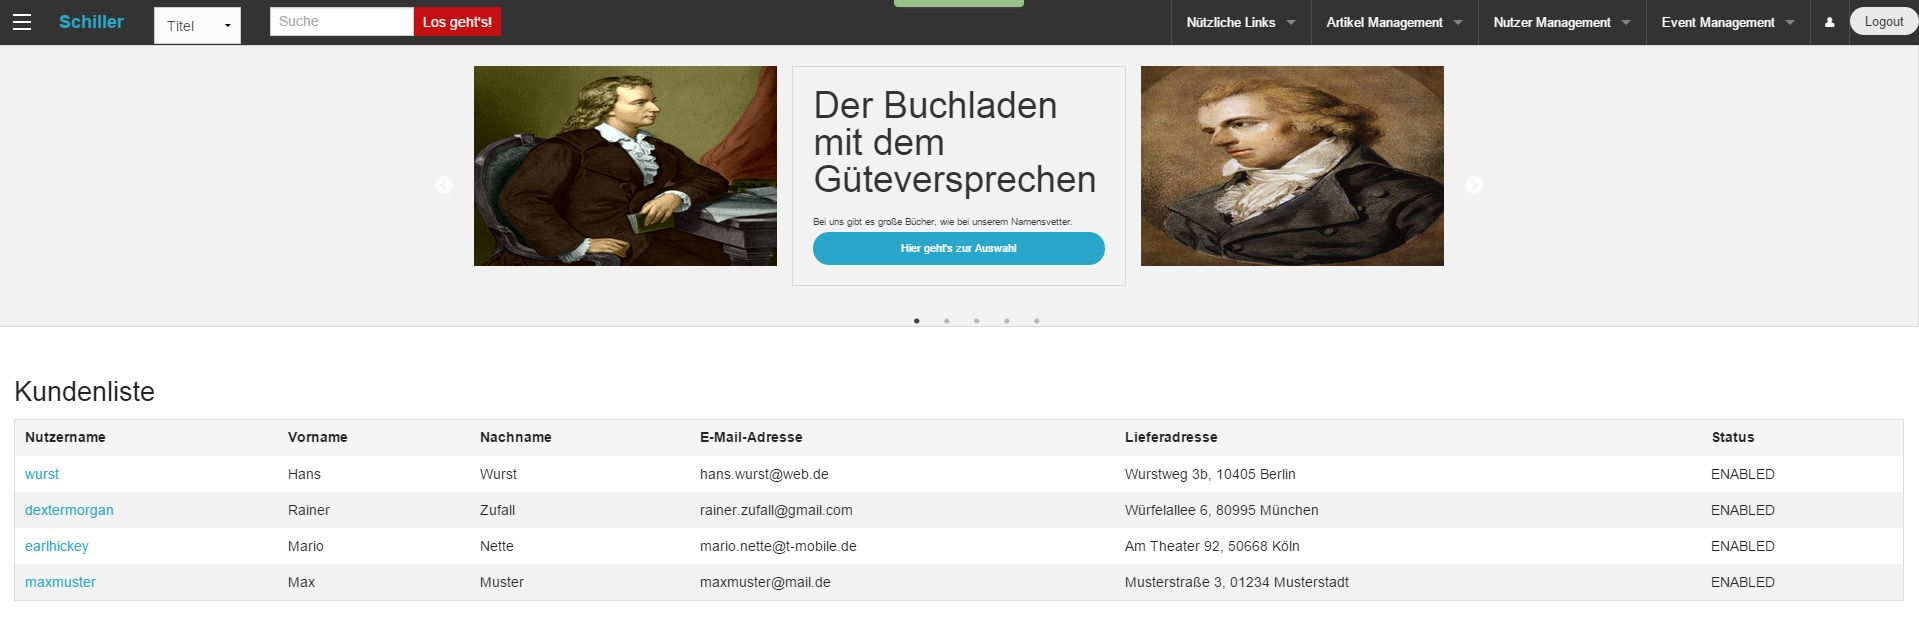
\includegraphics[width=1.0\textwidth]{Kundenliste.jpg}
\caption{Kundenübersicht}
\end{figure}
\smallskip

\begin{figure}[ht]
\centering
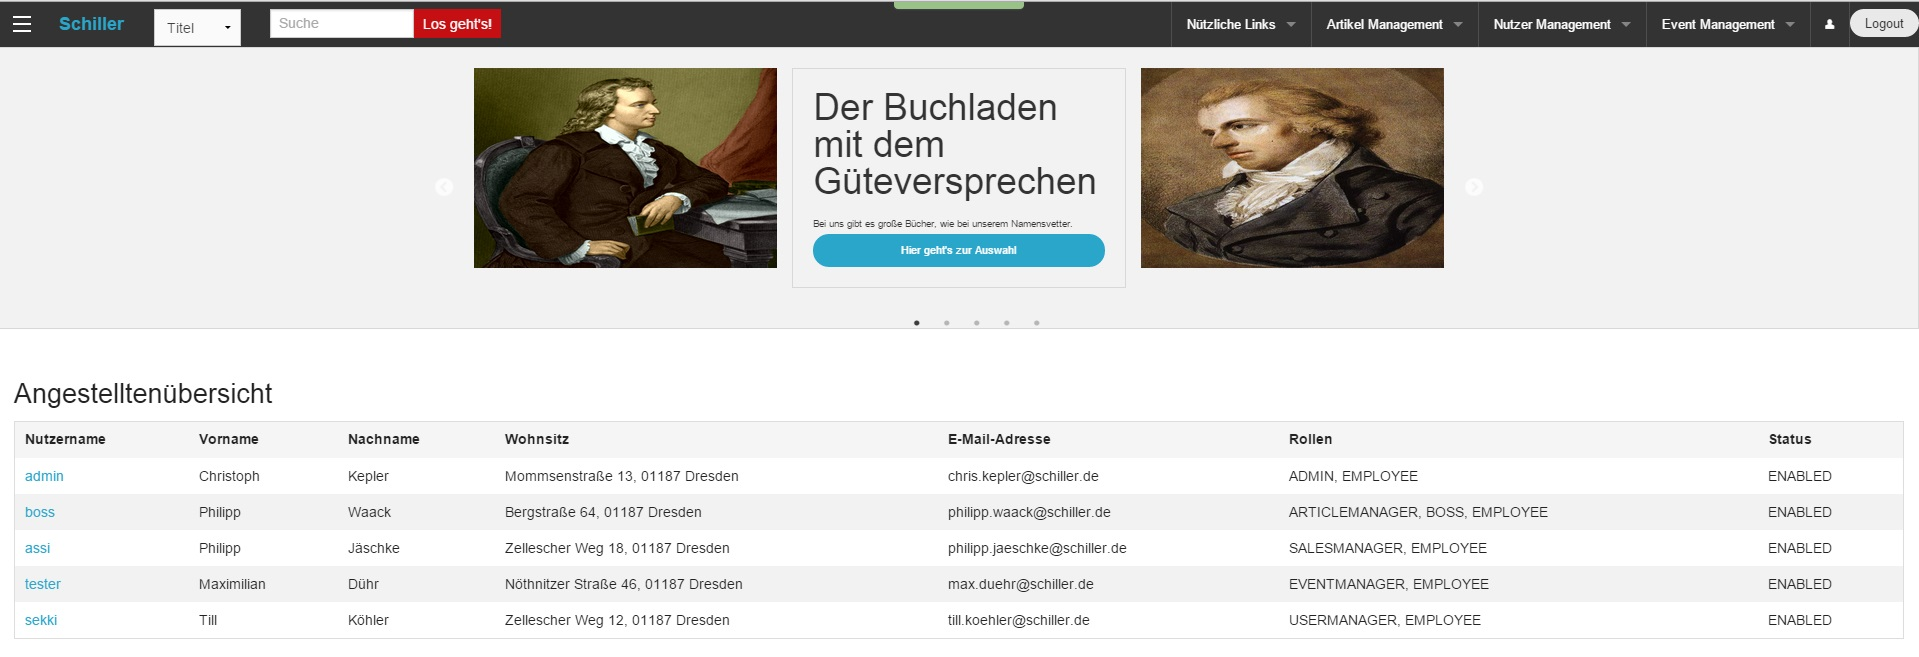
\includegraphics[width=1.0\textwidth]{Angestelltenliste.jpg}
\caption{Angestelltenübersicht}
\end{figure}
\smallskip

\FloatBarrier

\subsection{Fremde Profilansicht und -bearbeitung}

(ACHTUNG: Ein fremder Nutzer kann auch der aktuelle Nutzer selbst sein!) \\
Nutzer mit den Rollen ''Admin'', ''Boss'' und ''Usermanager'' gelangen durch Klicken auf den entsprechenden Nutzernamen in der Nutzerübersicht (siehe \ref{nutzer}) auf die Profilansichtsseite eines beliebigen anderen Nutzers. Das Layout entspricht dabei dem der eigenen Profilansicht (siehe \ref{profil}). \\
Zur Änderungsansicht der Profildaten gelangen Nutzer mit den Rollen ''Admin'' und ''Usermanager'' durch Klicken auf den entsprechenden Link über den Profildaten. Ein ''Boss'' (nicht ''Admin'' oder ''Usermanager'') kann diesen zwar anklicken, wird jedoch nicht weitergeleitet. Hier sind die aktuellen Daten des fremden Nutzeraccounts schon voreingetragen. Der aktuelle Nutzer kann diese nun ändern. Ist das Format der eingegebenen Daten nicht korrekt, dann erscheinen direkt nach der Eingabe Fehlermeldungen und die Profiländerung ist nicht möglich. Ist die E-Mail bereits vergeben, so erscheinen direkt nach Klicken auf den Button ''Neue Profildaten speichern'' Fehlermeldungen und es findet keine Profiländerung statt. Nur wenn alle eingegebenen Daten syntaktisch korrekt sind, werden die Profildaten des fremden Nutzers entsprechend geändert und der aktuelle Nutzer wird zur Profilansicht des fremden Nutzers weitergeleitet. \\
Zur Änderungsansicht der Accounteinstellungen gelangen Nutzer mit den Rollen ''Admin'' und ''Usermanager'' durch Klicken auf den entsprechenden Link über den Profildaten. Ist der aktuelle Nutzer kein ''Admin'' und möchte die Accounteinstellungen eines fremden Nutzers mit der Rolle ''Admin'' oder seine eigenen Accounteinstellungen ändern, so wird er nach Klicken des entsprechenden Links nicht weitergeleitet. In allen anderen Fällen wird der Nutzer nach Klicken des Links auf die entsprechende Seite weitergeleitet. Hier werden der aktuelle Status und der aktuelle Rollen angezeigt. Der aktuelle Nutzer kann nun das Profil des fremden Nutzers deaktivieren (wenn der fremde Nutzeraccount aktiviert ist) oder aktivieren (wenn der fremde Nutzeraccount deaktiviert ist). Ein Nutzer mit der Rolle ''Admin'' kann nicht deaktiviert werden. Außerdem kann der Nutzer hier dem fremden Account eine Rolle hinzufügen (wenn er diese noch nicht besitzt) oder eine Rolle von von dem Account entfernen (wenn er diese bereits besitzt). Ist der fremde Nutzer der letzte Nutzer mit der Rolle ''Admin'', so kann die Rolle ''Admin'' nicht entfernt werden. Es sind bei der Rollenänderung nur diejenigen Rollen auswählbar, welche hinzufügbar oder entfernbar sind. 

\begin{figure}[ht]
\centering
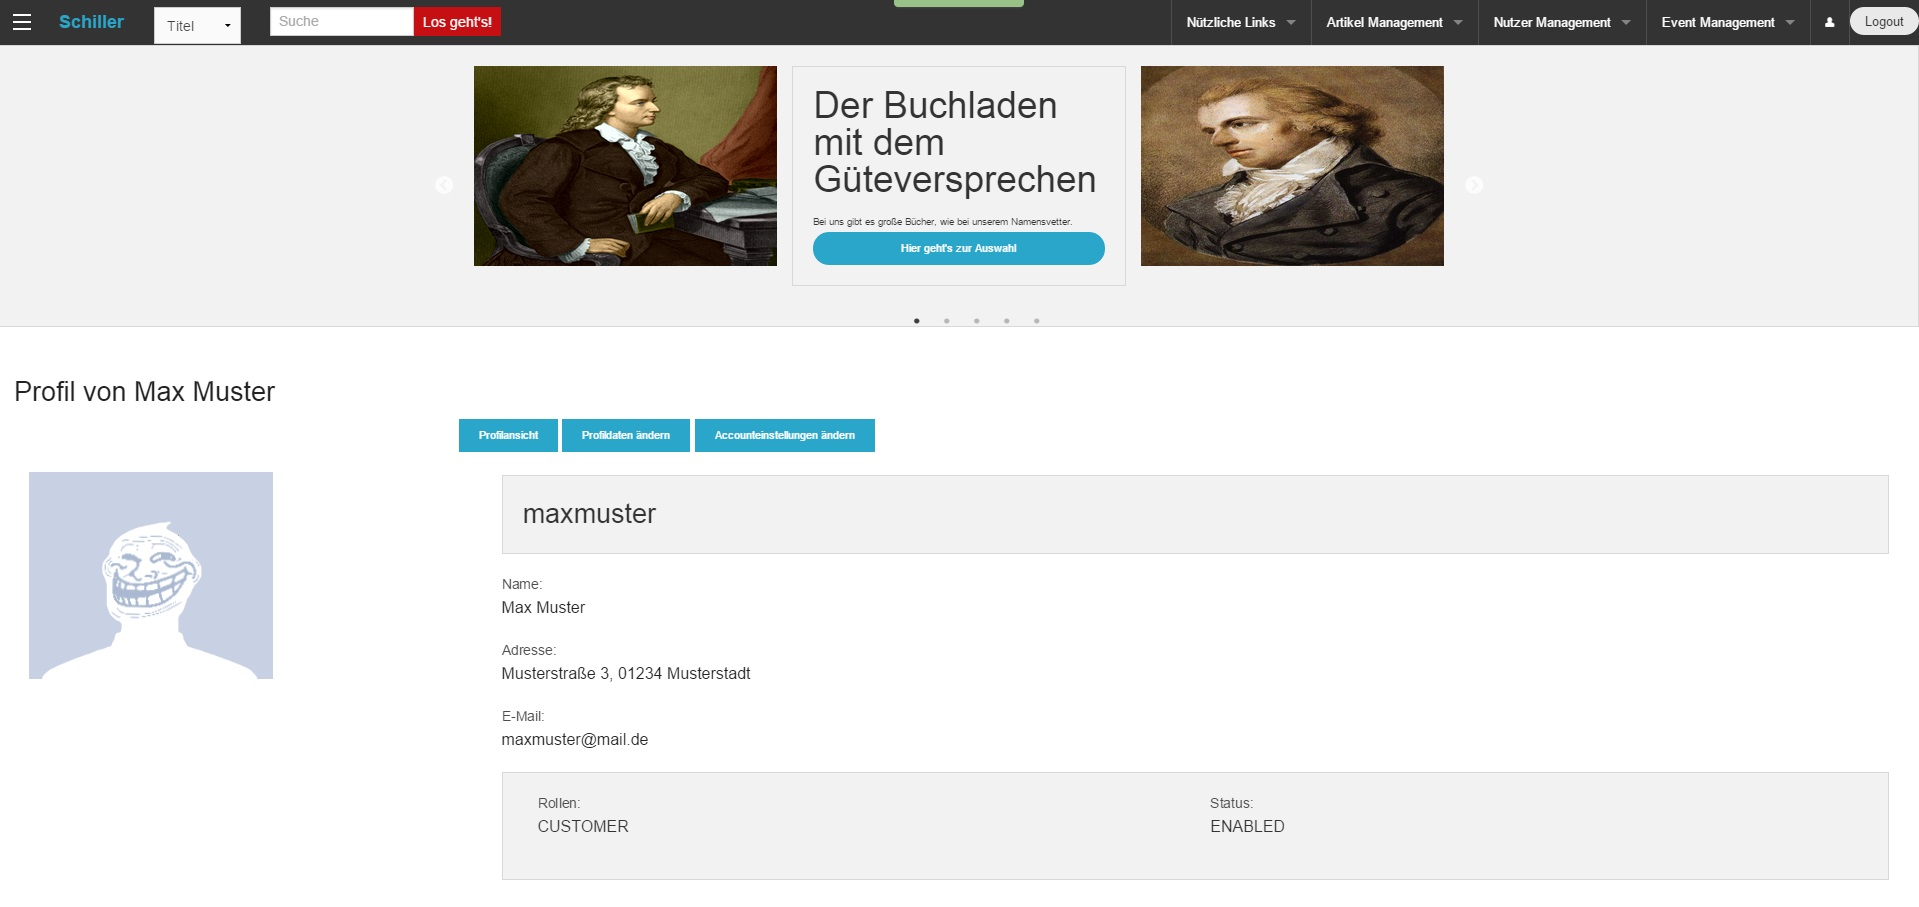
\includegraphics[width=1.0\textwidth]{Profil_fremd.jpg}
\caption{Fremde Profilansicht}
\end{figure}
\smallskip

\begin{figure}[ht]
\centering
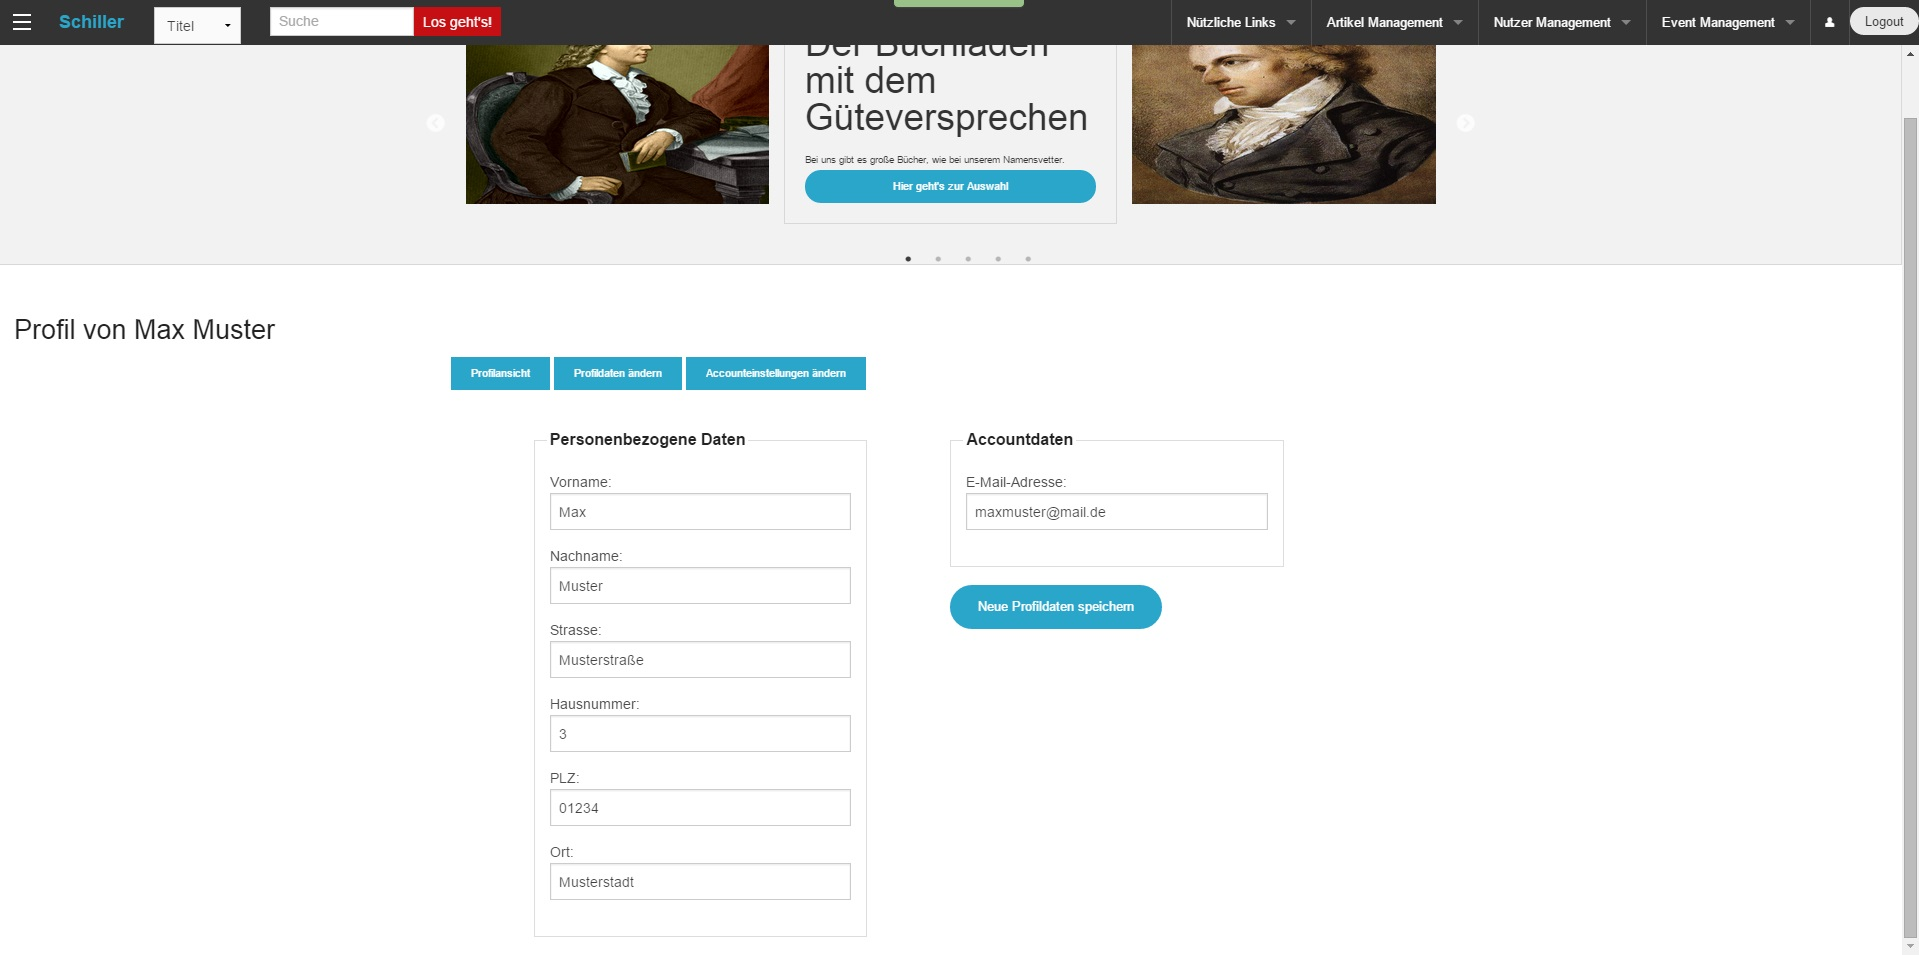
\includegraphics[width=1.0\textwidth]{Profilaenderung_fremd.jpg}
\caption{Profiländerung des fremden Profils}
\end{figure}
\smallskip

\begin{figure}[ht]
\centering
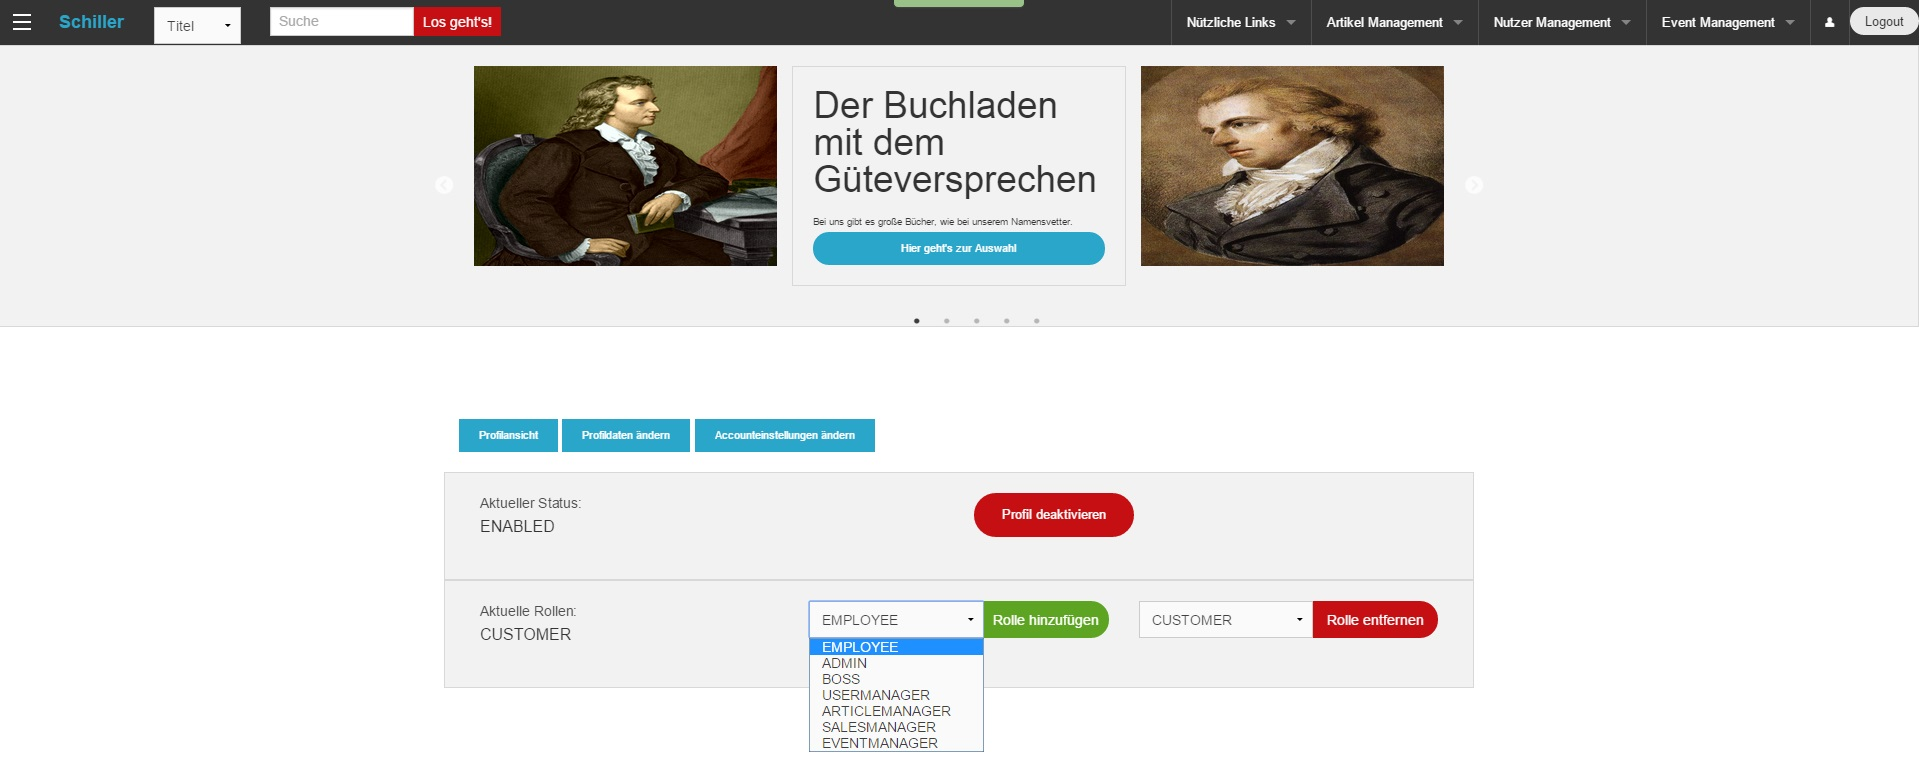
\includegraphics[width=1.0\textwidth]{Accountdaten.jpg}
\caption{Änderung der Accounteinstellungen}
\end{figure}
\smallskip

\FloatBarrier

\subsection{Anlegen eines neuen Nutzers}

Nutzer mit den Rollen ''Admin'' und ''Usermanager'' gelangen durch Klicken auf den Link ''Nutzer erstellen'' in der Dropdownliste ''Nutzer Management'' zum Erstellungsformular für einen neuen Nutzer. \\
Hier müssen verschiedene personenbezogene Daten (Vorname, Nachname, Straße, Nummer, PLZ, Ort) und Accountdaten (Nutzername, E-Mail, Passwort, Passwortwiederholung) angegeben werden. Außerdem muss der aktuelle Nutzer auswählen, ob der neue Nutzer ein Kunde (Rolle ''Customer'') oder ein Angestellter (Rolle ''Employee'') sein soll. Ist das Format der eingegebenen Daten nicht korrekt, dann erscheinen direkt nach Eingabe Fehlermeldungen und die Registrierung ist nicht möglich. Sind Nutzername bzw. E-Mail bereits vergeben, so erscheinen direkt nach Klicken auf den Button ''Registrieren'' Fehlermeldungen und es findet keine Registrierung statt. Nur wenn alle eingegebenen Daten syntaktisch korrekt sind, wird der neue Nutzer mit den angegebenen Daten als Kunde bzw. Angestellter registriert.

\begin{figure}[ht]
\centering
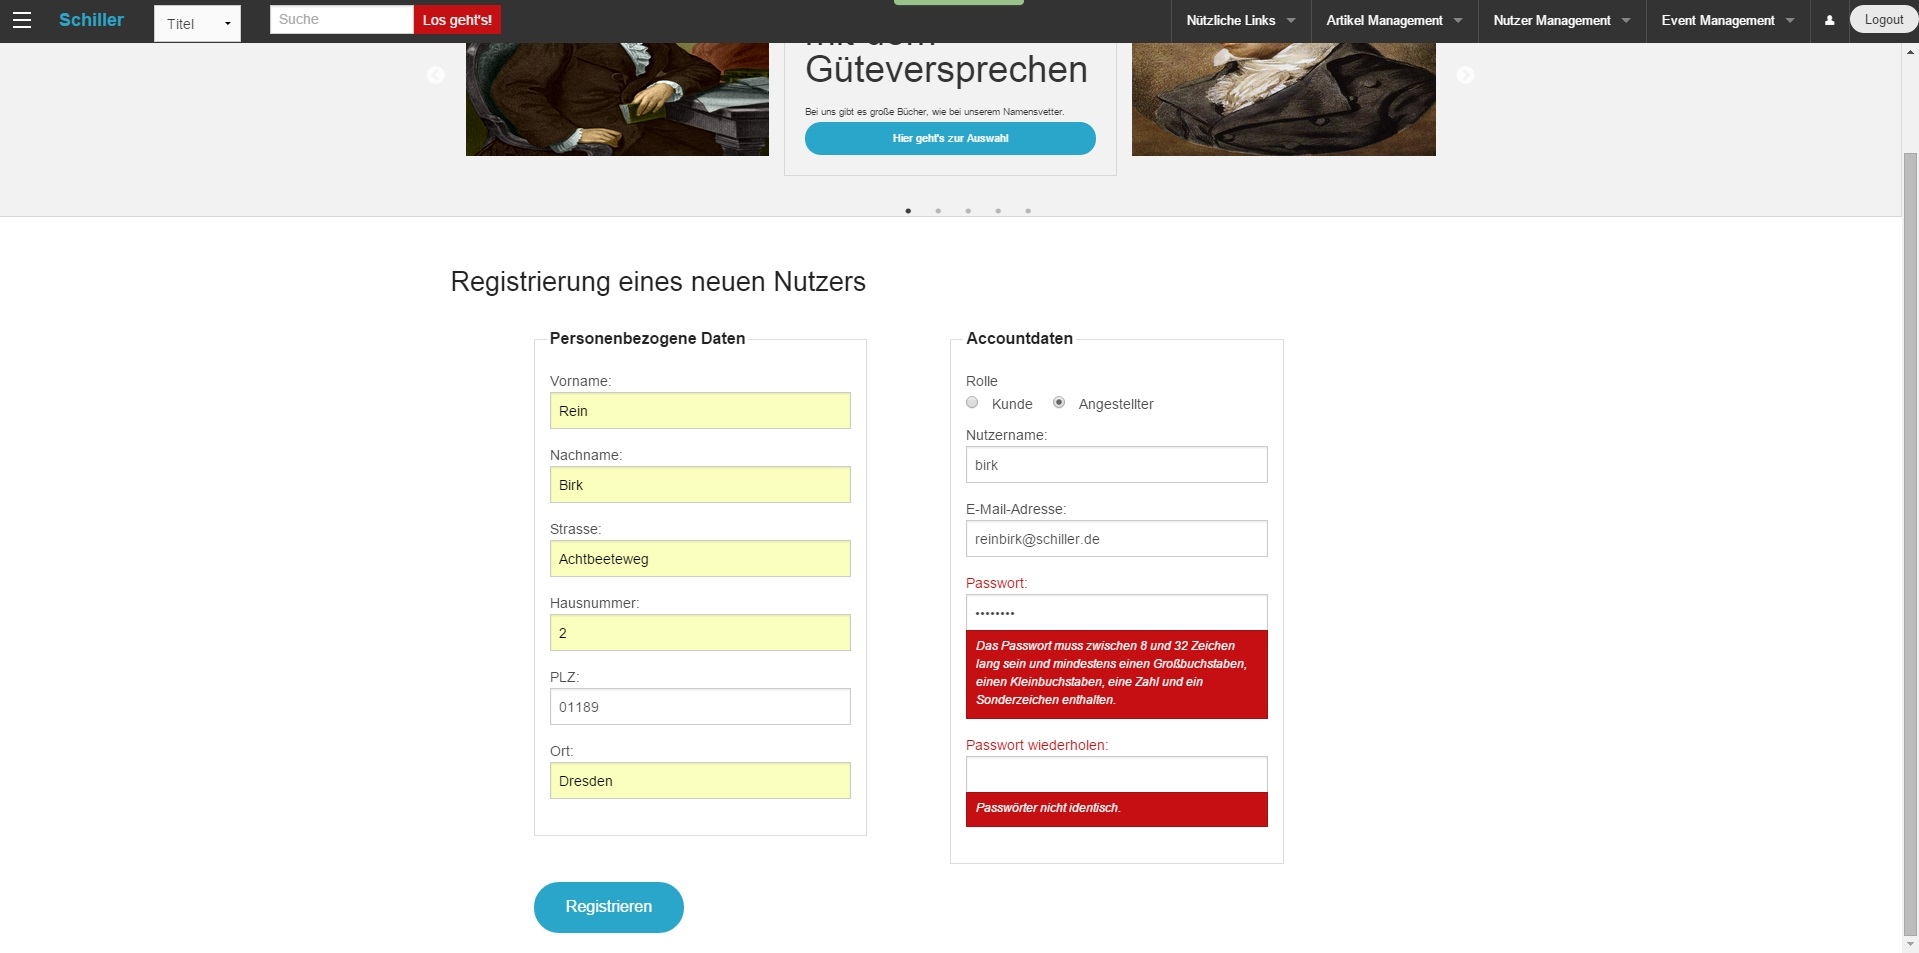
\includegraphics[width=1.0\textwidth]{NeuerNutzer.jpg}
\caption{Registrierung eines neuen Angestellten}
\end{figure}
\smallskip

\FloatBarrier

\subsection{Bearbeitung von Artikeln} \label{artikeländerung}

Nutzer mit den Rollen ''Admin'' und ''Articlemanager'' gelangen über die Detailansicht für Artikel (siehe \ref{detail}) zum jeweiligen Änderungsformular für Artikel durch Klicken auf den Link ''Artikel ändern'' direkt über den Artikeldaten. \\
Hier sind die aktuellen Daten des Artikels schon voreingetragen. Der Nutzer kann diese nun ändern. Ist das Format der eingegebenen Daten nicht korrekt, dann erscheinen direkt nach der Eingabe Fehlermeldungen und die Änderung des Artikels ist nicht möglich. Nur wenn alle eingegebenen Daten syntaktisch korrekt sind, werden Artikeldaten entsprechend geändert und der Nutzer wird zur Ansichtsseite des Artikels weitergeleitet. \\
Außerdem können Nutzer mit den Rollen ''Admin'' und ''Articlemanager'' durch Klicken auf den Link ''Artikel löschen'' direkt über den Artikeldaten den angezeigten Artikel löschen. Tut man dies gelangt man zunächst auf eine Bestätigungsseite. Durch Klicken auf ''Lösche Artikel'' kann der Nutzer die Löschung des Artikels bestätigen.

\begin{figure}[ht]
\centering
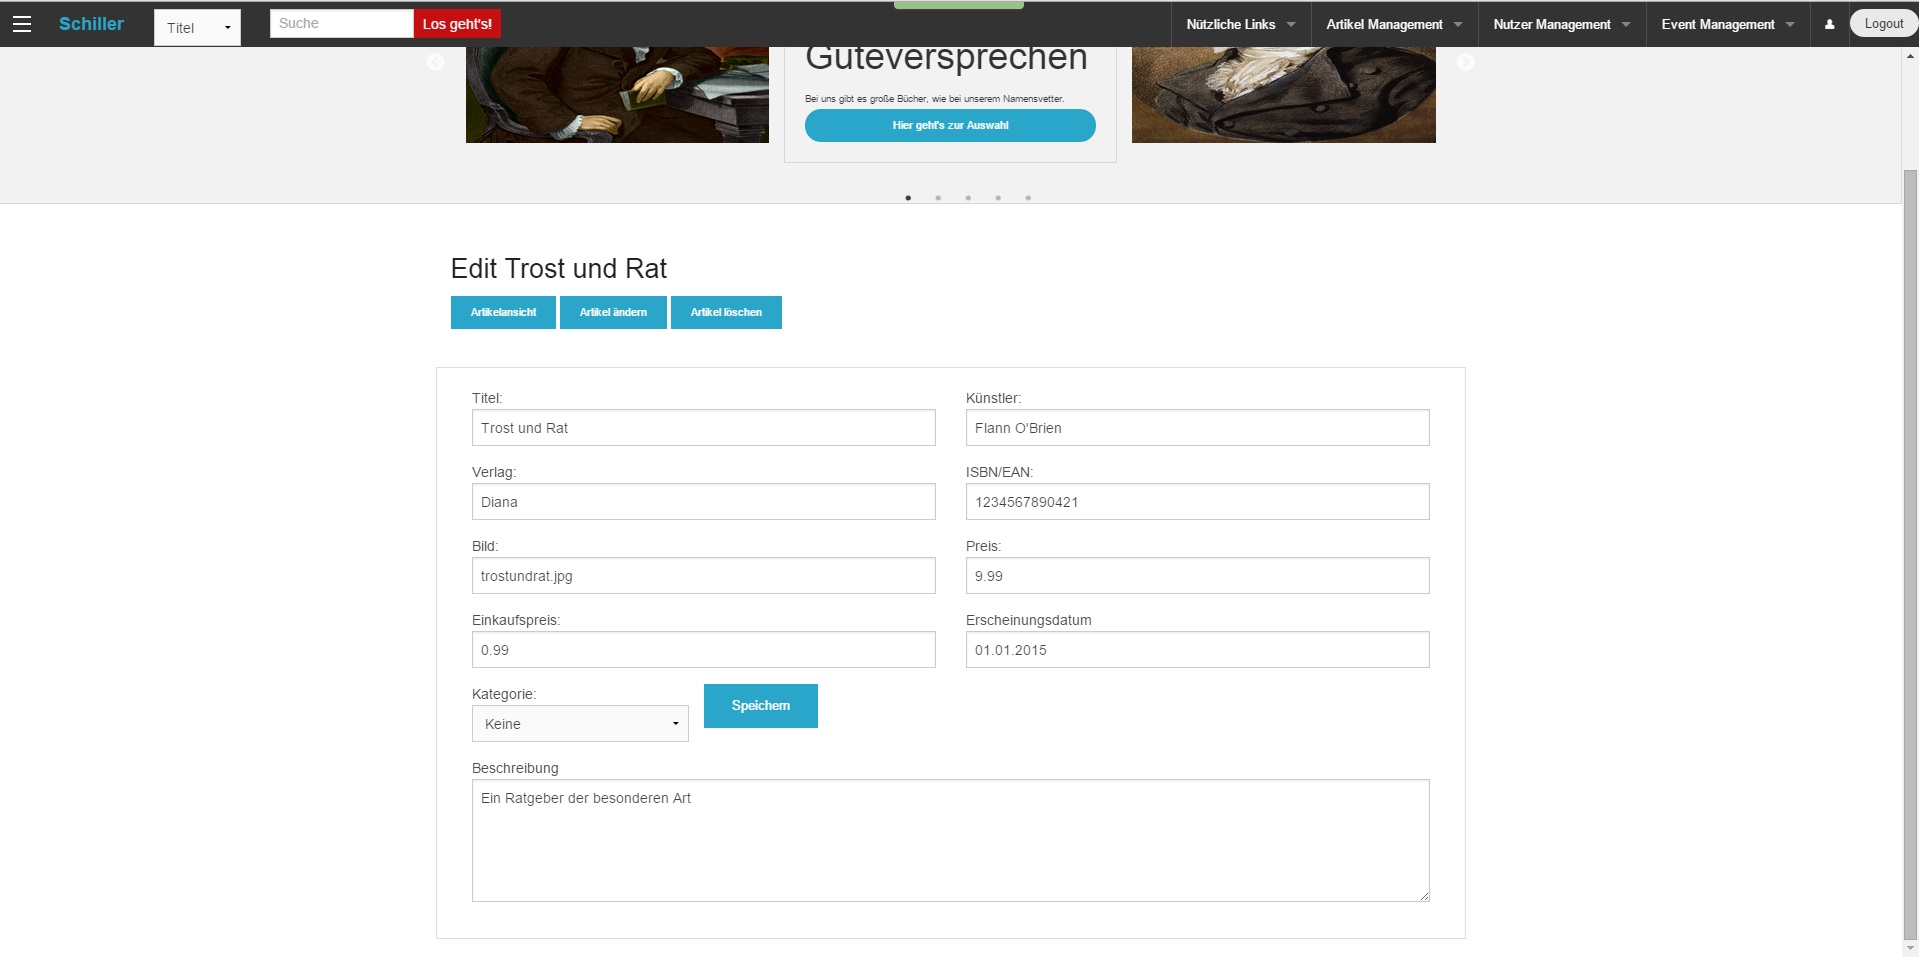
\includegraphics[width=1.0\textwidth]{Artikelaenderung.jpg}
\caption{Änderung eines Artikels}
\end{figure}
\smallskip

\FloatBarrier

\subsection{Anlegen neuer Artikel}

Nutzer mit den Rollen ''Admin'' und ''Articlemanager'' gelangen durch Klicken auf die Links ''Buch anlegen'', ''CD anlegen'' bzw. ''DVD anlegen'' in der Dropdownliste ''Artikel Management'' zum Erstellungsformular für ein neues Buch, eine neue CD bzw. eine neue DVD. \\
Hier müssen verschiedene Daten (bei Buch: Titel, Autor, Verlag, ISBN, Preis, Einkaufspreis, Erscheinungsdatum, Kategorie, Bildpfad und Artikelbeschreibung) des Artikels angegeben werden. Ist das Format der eingegebenen Daten nicht korrekt, dann erscheinen direkt nach Eingabe Fehlermeldungen und das Hinzufügen des neuen Artikels ist nicht möglich. Nur wenn alle eingegebenen Daten syntaktisch korrekt sind, wird der Artikel nach Klicken des entsprechenden Buttons mit den angegebenen Daten hinzugefügt.

\begin{figure}[ht]
\centering
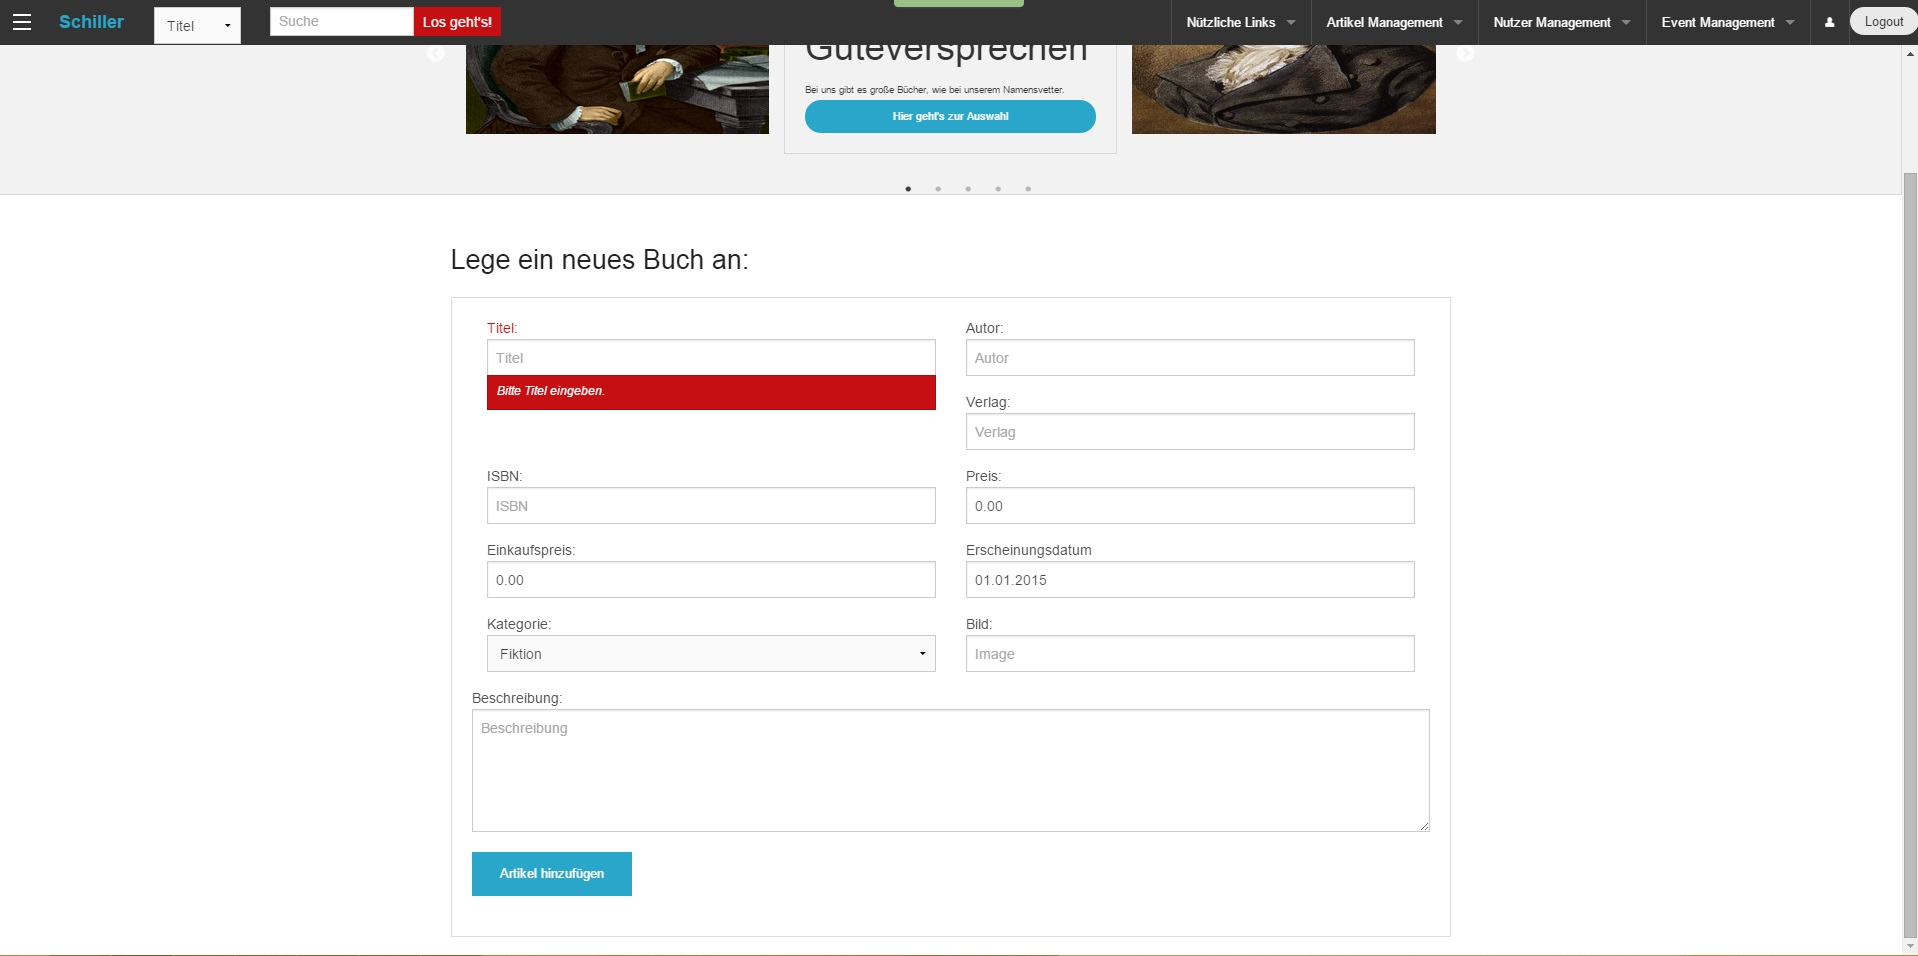
\includegraphics[width=1.0\textwidth]{NeuerArtikel.jpg}
\caption{Anlegen eines neuen Artikels}
\end{figure}
\smallskip

\FloatBarrier

\subsection{Bearbeitung der Kategorien}

Nutzer mit den Rollen ''Admin'' und ''Articlemanager'' gelangen durch Klicken auf den Link ''Kategorien bearbeiten'' in der Dropdownliste ''Artikel Management'' zur Bearbeitungsansicht für die Artikelkategorien. \\
Hier kann der Nutzer durch Eingabe der Kategoriebezeichnung, Auswahl des Kategorietyps (''Buch'', ''CD'' oder ''DVD'') in der oberen Dropdownliste und Klicken des Buttons ''Hinzufügen'' eine neue Kategorie hinzufügen. Ist das Eingabefeld der Artikelbezeichnung leer, so ist das Hinzufügen der Kategorie nicht möglich. Außerdem kann der Nutzer durch Auswahl der Kategorie in der unteren Dropdown-Liste und Klicken des Buttons ''Entfernen'' eine bereits vorhandene Kategorie löschen. 

\begin{figure}[ht]
\centering
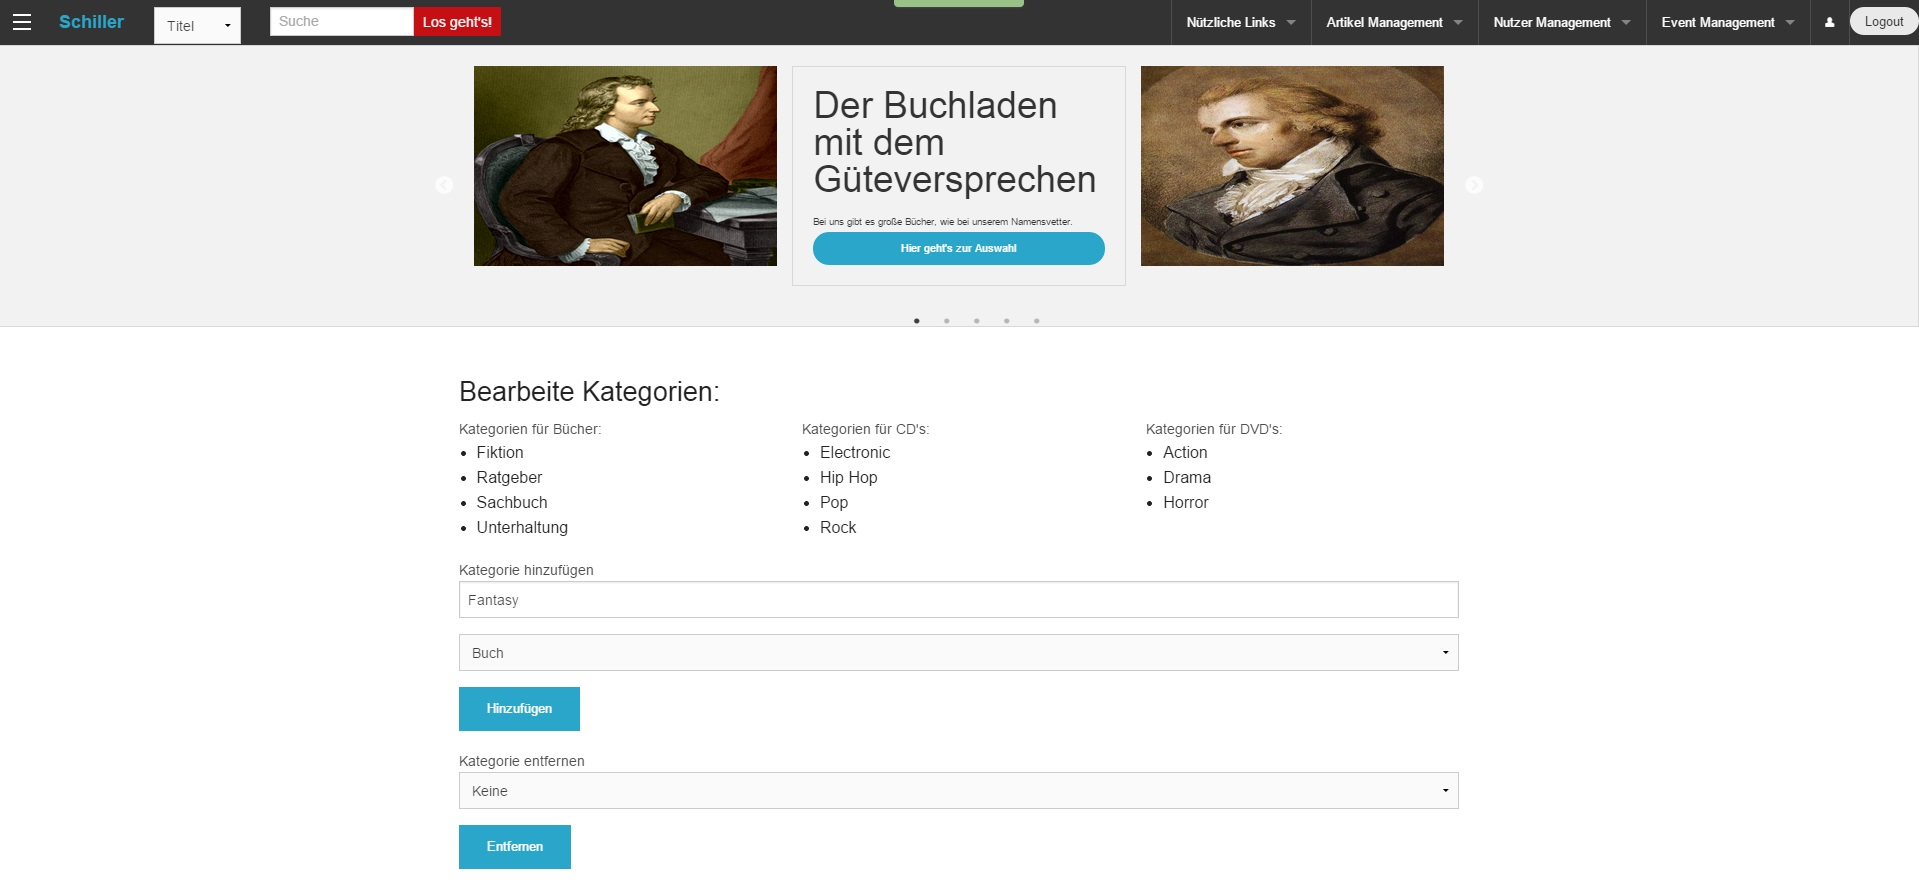
\includegraphics[width=1.0\textwidth]{Kategorien.jpg}
\caption{Bearbeitung der Kategorien}
\end{figure}
\smallskip

\FloatBarrier

\subsection{Bestellungsübersicht}

Nutzer mit den Rollen ''Admin'' und ''Salemanager'' gelangen durch Klicken auf den Link ''Bestellungsübersicht'' in der Dropdownliste ''Nützliche Links'' zur Bestellungsübersicht. \\
Hier erhält der Nutzer Überblick über zwei Tabellen mit Bestellungen. Auf der linken Seite sind alle offenen Bestellungen (inkl. Rechnungsnummer und gezahltem Betrag) aufgeführt. Der Nutzer kann durch Klicken des Buttons ''Versenden'' die Bestellung abschließen. Sobald die Bestellung abgeschlossen wurde, wird sie aus der linken Tabelle entfernt und in die rechte Tabelle eingefügt. Hier werden werden alle abgeschlossen Bestellungen (inkl. Rechnungsnummer und gezahltem Betrag) angezeigt. Hinter allen Bestellungen(egal ob offen oder abgeschlossen) wird ein weiterer Link ''Detailansicht'' angezeigt. Durch Klicken dieses Links wird der Nutzer zur Detailansicht der Bestellung weitergeleitet. Diese entspricht von Layout und Funktionalität her der Detailansicht wie in \ref{bestellung}.

\begin{figure}[ht]
\centering
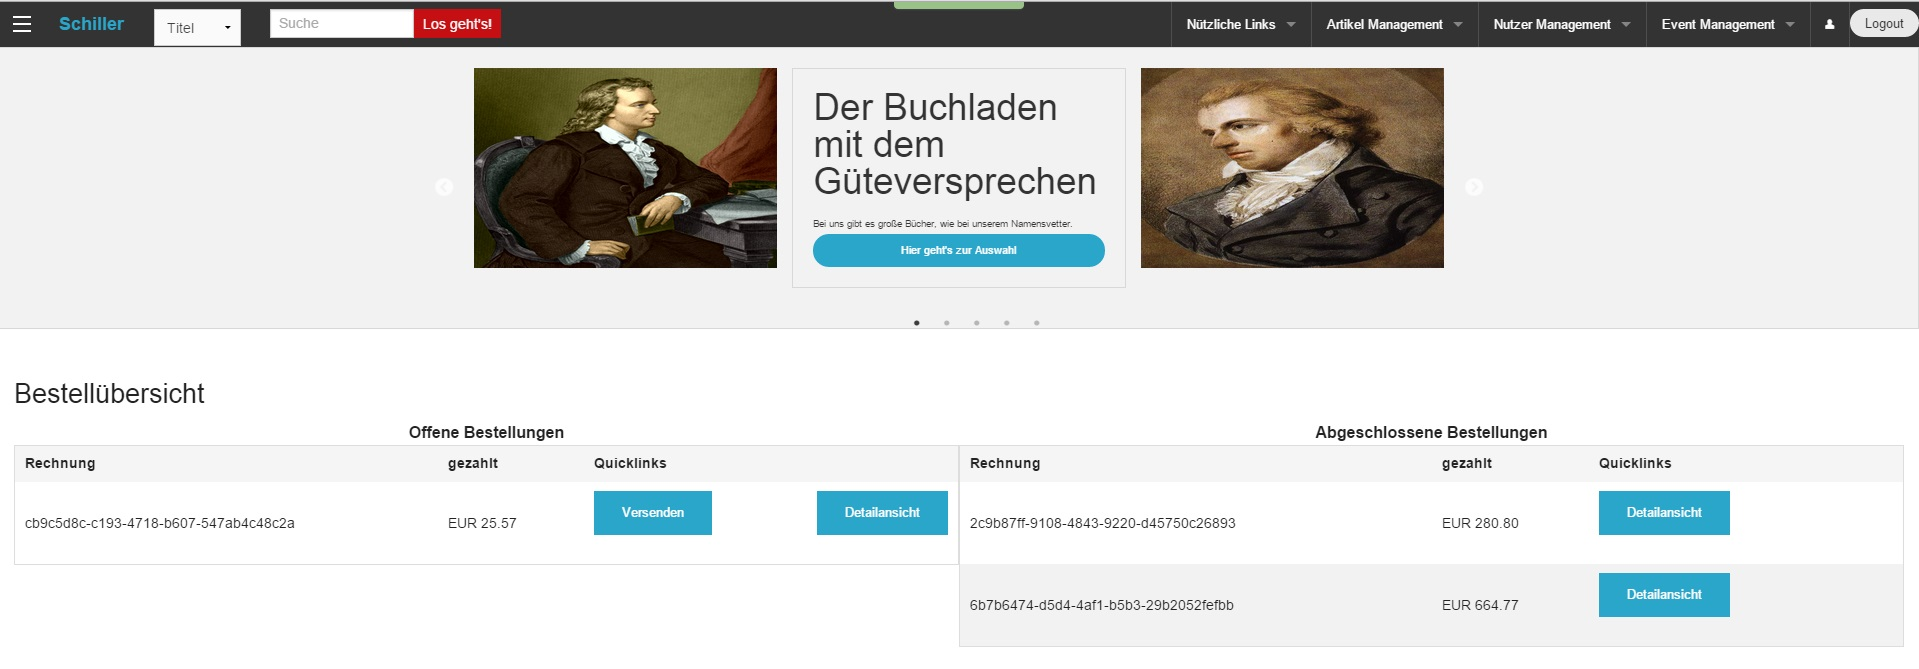
\includegraphics[width=1.0\textwidth]{Bestellungsansicht.jpg}
\caption{Bestellungsübersicht}
\end{figure}
\smallskip

\FloatBarrier

\subsection{Lagerübersicht}

Nutzer mit den Rollen ''Admin'' und ''Salemanager'' gelangen durch Klicken auf den Link ''Lagerübersicht'' in der Dropdownliste ''Nützliche Links'' zur Lagerübersicht. \\
Hier wird eine Liste aller Artikel mit der jeweiligen sich im Lager befindlichen Anzahl des Artikels angezeigt. Hier kann der Nutzer durch Eingabe einer positiven ganzen Zahl in das Eingabefeld und anschließendes Klicken des Buttons ''Nachbestellen'' eine gewünschte Anzahl des gewählten Artikels nachbestellen. Diese wird sofort im Lager hinzugefügt und in die Statistiken mit einbezogen.

\begin{figure}[ht]
\centering
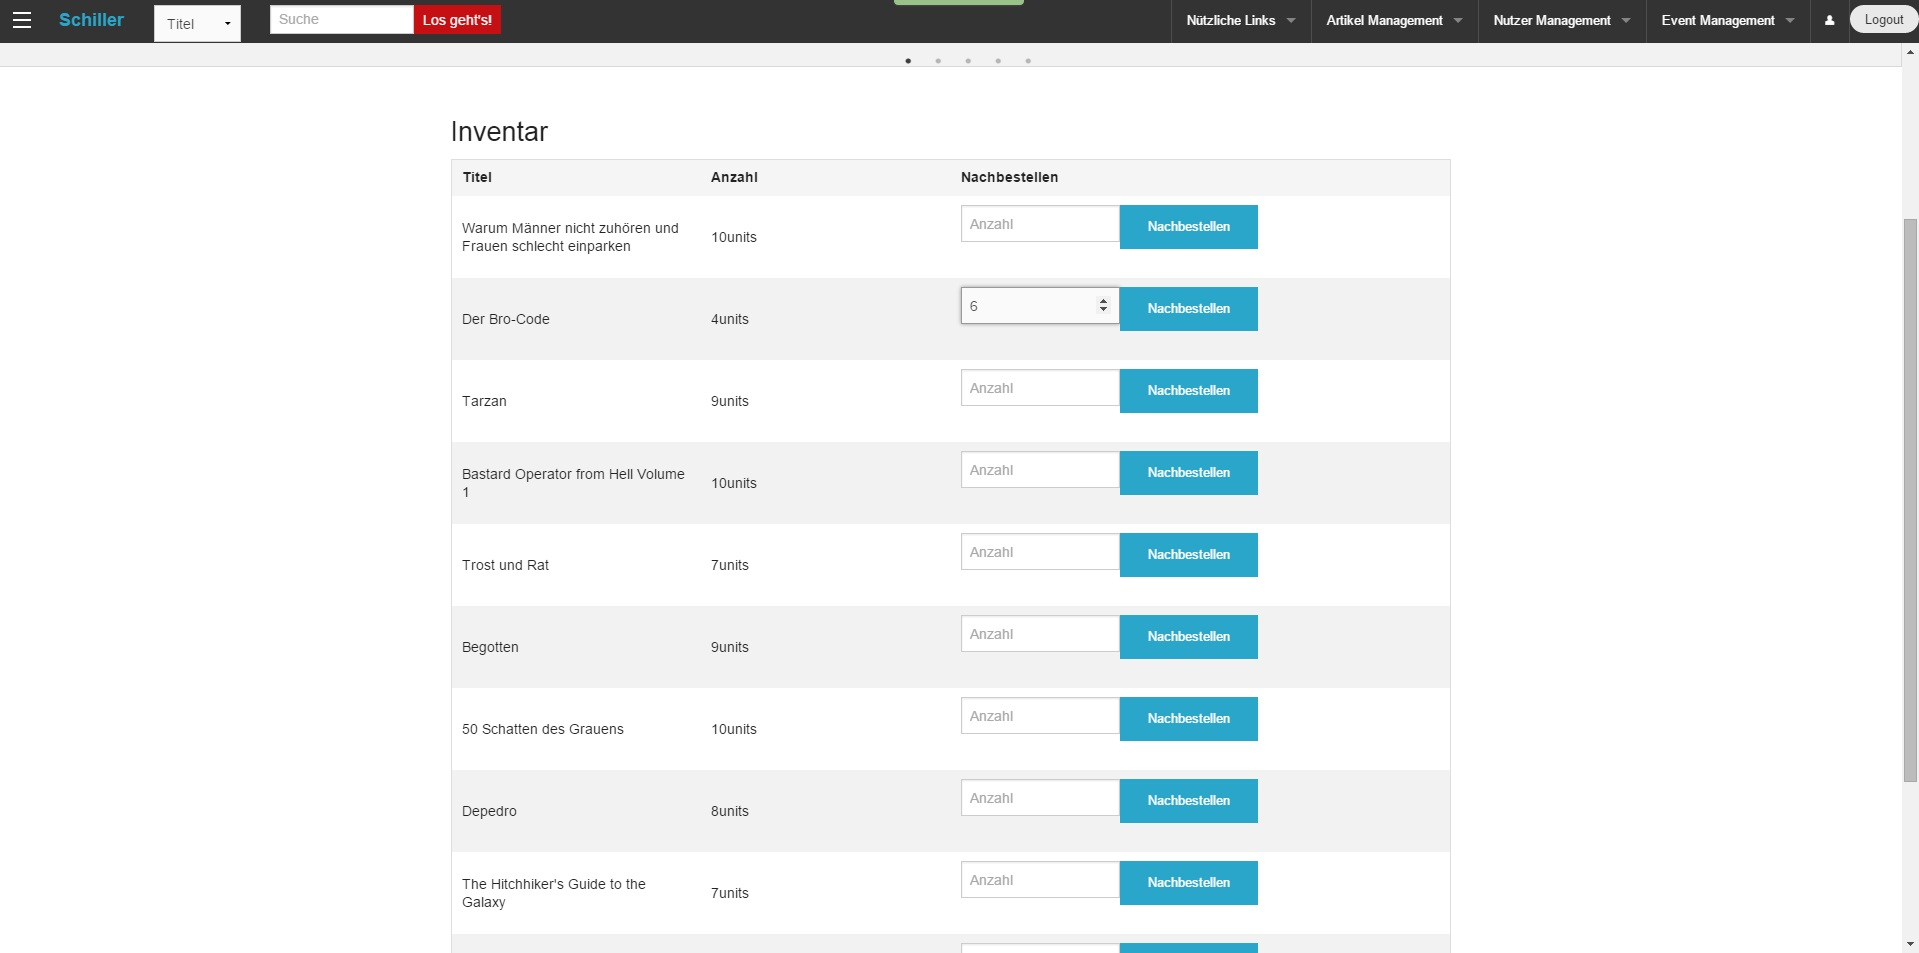
\includegraphics[width=1.0\textwidth]{Lager.jpg}
\caption{Lagerübersicht}
\end{figure}
\smallskip

\FloatBarrier

\subsection{Ansicht der Statistiken}

Nutzer mit den Rollen ''Admin'' und ''Salemanager'' gelangen durch Klicken auf den Link ''Statistiken'' in der Dropdownliste ''Nützliche Links'' zur Ansicht der Statistiken. \\
Hier erhält der Nutzer Überblick über zwei Bilanztabellen. Auf der linken Seite werden für jeden Artikel jeweils Titel, Anzahl der verkauften Exemplare in der letzten Woche und Einnahmen in der letzten Woche aufgeführt. Auf der rechten Seite werden für jeden Artikel jeweils Titel, Anzahl der nachbestellten Exemplare in der letzten Woche und Ausgaben in der letzten Woche aufgeführt. Unter der Tabelle werden alle Einnahmen aus Sitzplatzreservierungen für Events angezeigt. Außerdem findet der Nutzer hier die wöchentlichen Einnahmen, Ausgaben und den wöchentlichen Profit aller Artikel, sowie die Gesamteinnahmen, -ausgaben und den Gesamtprofit seit Bestehen der Buchhandlung Schiller im Überblick.

\begin{figure}[ht]
\centering
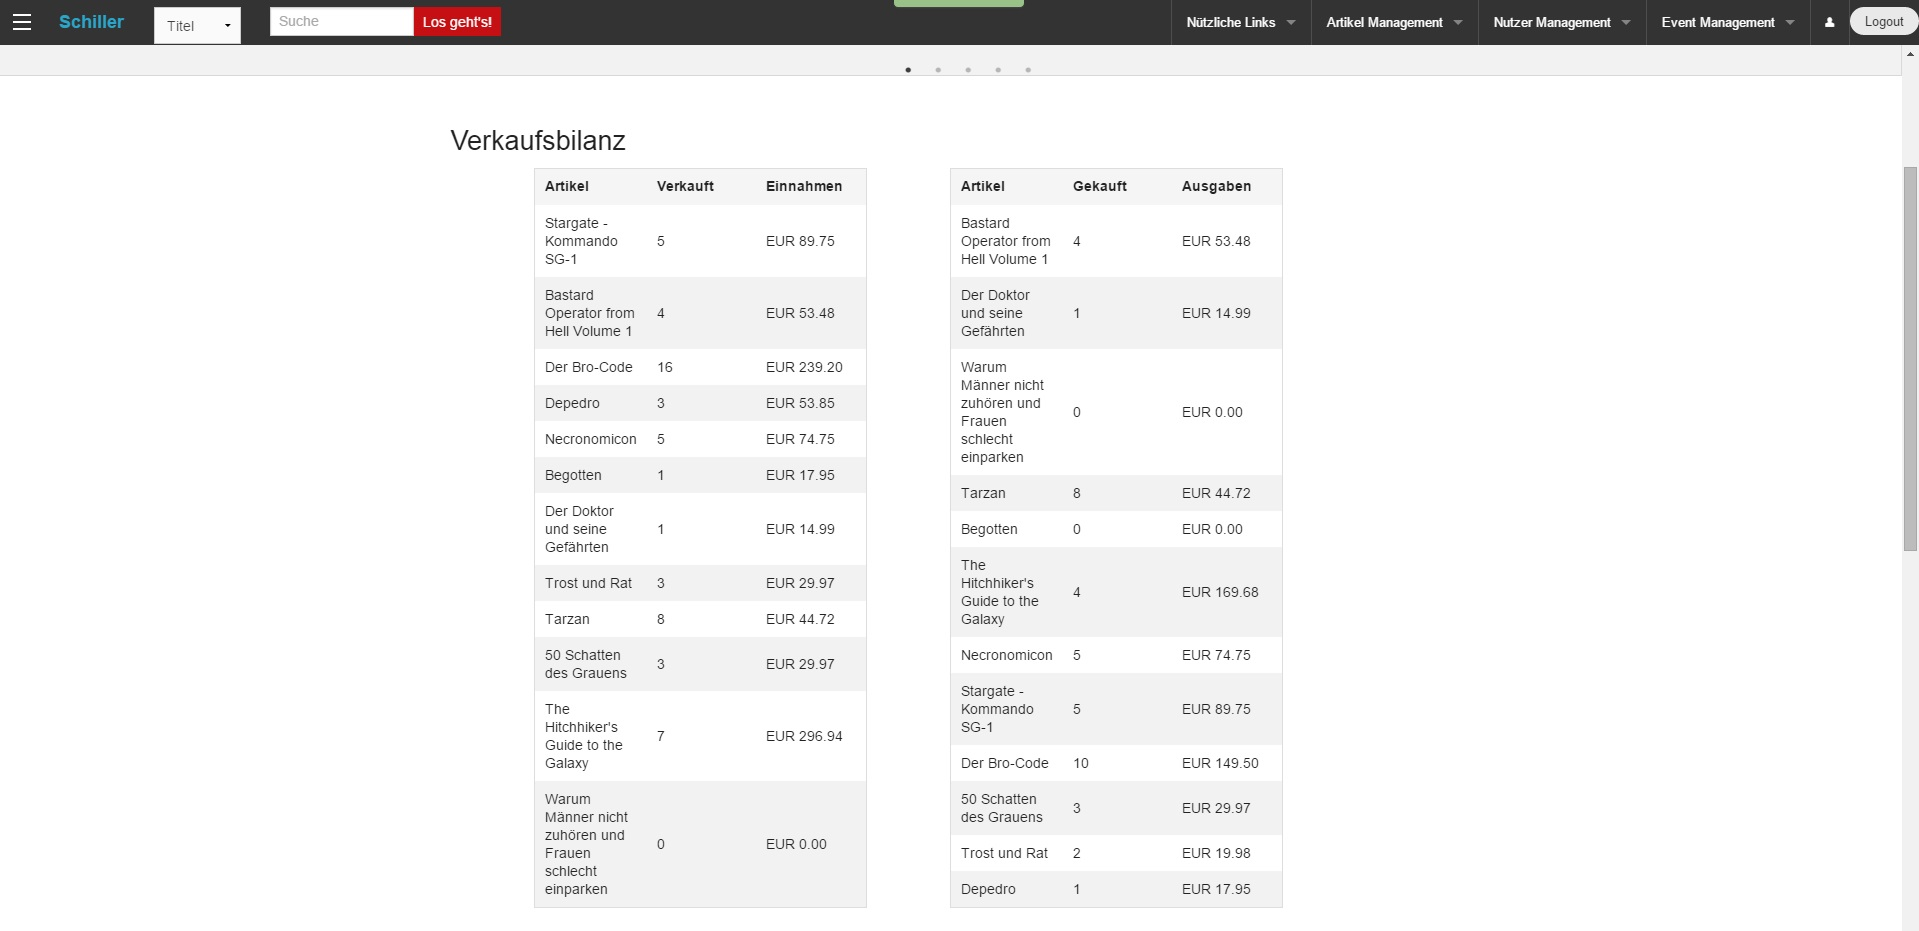
\includegraphics[width=1.0\textwidth]{Statistiken1.jpg}
\caption{Artikeltabelle der Statistiken}
\end{figure}
\smallskip

\begin{figure}[ht]
\centering
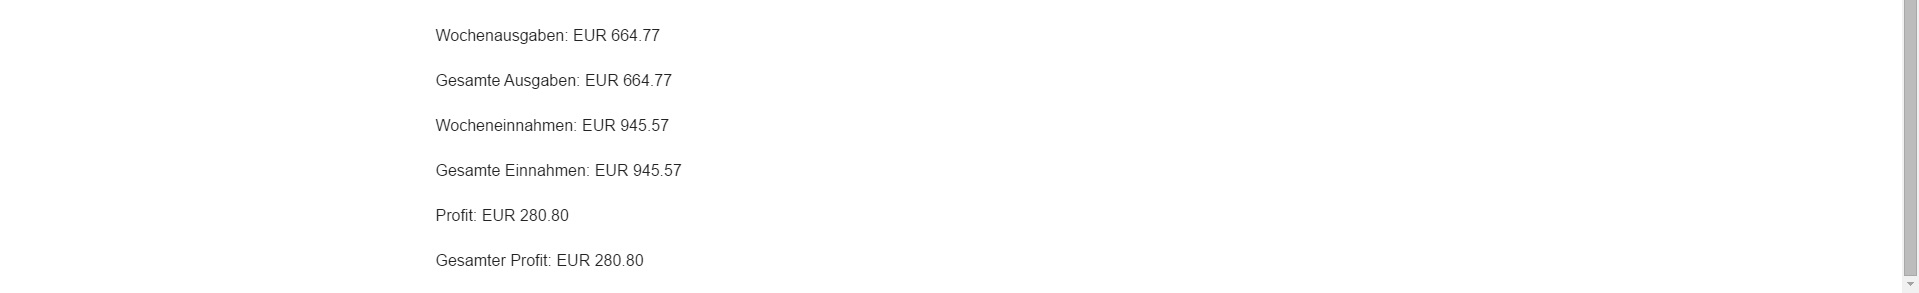
\includegraphics[width=1.0\textwidth]{Statistiken2.jpg}
\caption{Gesamtsummen der Statistiken}
\end{figure}
\smallskip

\FloatBarrier

\subsection{Bearbeitung der Events}

Nutzer mit den Rollen ''Admin'' und ''Eventmanager'' gelangen durch Klicken auf den Link ''Events bearbeiten'' in der Dropdownliste ''Event Management'' zum Bearbeitungsansicht für die Events. \\
Im oberen Teil der Seite kann ein neues Event angelegt werden. Hier müssen verschiedene Daten (Datum, Uhrzeiten für Anfang und Ende, Veranstaltungsname und Raum) des Events angegeben oder in Dropdownlisten ausgewählt werden. Ist das Format der eingegebenen Daten nicht korrekt, dann erscheinen direkt nach Eingabe Fehlermeldungen und das Hinzufügen des neuen Events ist nicht möglich. Nur wenn alle eingegebenen Daten syntaktisch korrekt sind, wird das Event nach Klicken des entsprechenden Buttons mit den angegebenen Daten hinzugefügt.
Im unteren Teil der Seite sind in einer Tabelle alle bisherigen Events (inkl. Datum, Uhrzeiten für Anfang und Ende, Veranstaltungsname, Raumnummer, Raumname) aufgeführt. Hier kann der Nutzer Events, durch Klicken des Buttons ''Löschen'' hinter dem entsprechenden Event, löschen.

\begin{figure}[ht]
\centering
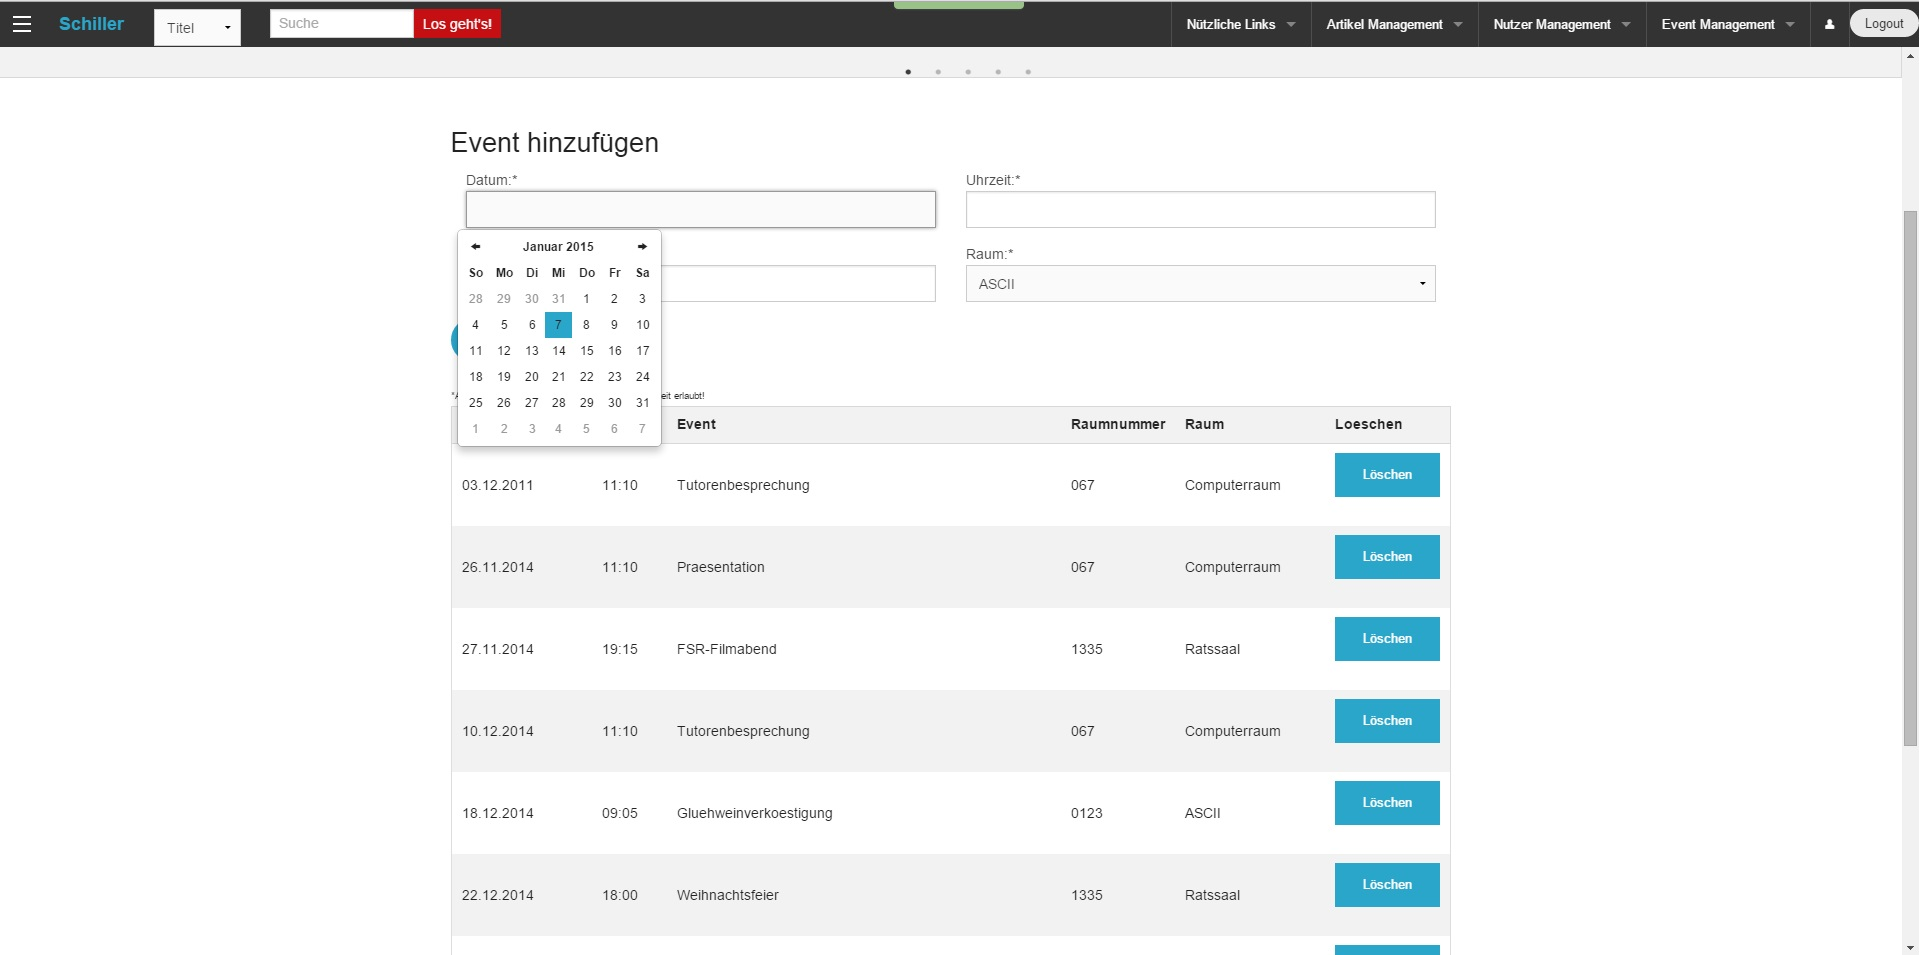
\includegraphics[width=1.0\textwidth]{Events.jpg}
\caption{Eventbearbeitung}
\end{figure}
\smallskip

\FloatBarrier

\subsection{Bearbeitung der Räume}

Nutzer mit den Rollen ''Admin'' und ''Eventmanager'' gelangen durch Klicken auf den Link ''Räume bearbeiten'' in der Dropdownliste ''Event Management'' zum Bearbeitungsansicht für die Räume. \\
Im oberen Teil der Seite kann ein neuer Raum angelegt werden. Hier müssen verschiedene Daten (Name, Nummer und Anzahl der Stühle) des Raumes angegeben werden. Ist das Format der eingegebenen Daten nicht korrekt, dann erscheinen direkt nach Eingabe Fehlermeldungen und das Hinzufügen des neuen Raumes ist nicht möglich. Nur wenn alle eingegebenen Daten syntaktisch korrekt sind, wird der Raum nach Klicken des entsprechenden Buttons mit den angegebenen Daten hinzugefügt.
Im unteren Teil der Seite sind in einer Tabelle alle bisherigen Räume (inkl. Raumname, Raumnummer und Anzahl der Sitzplätze) aufgeführt. Unter der Tabelle kann der Nutzer Räume, durch Auswahl in der Dropdownliste und anschließendes Klicken des Buttons ''Raum entfernen'', löschen.

\begin{figure}[ht]
\centering
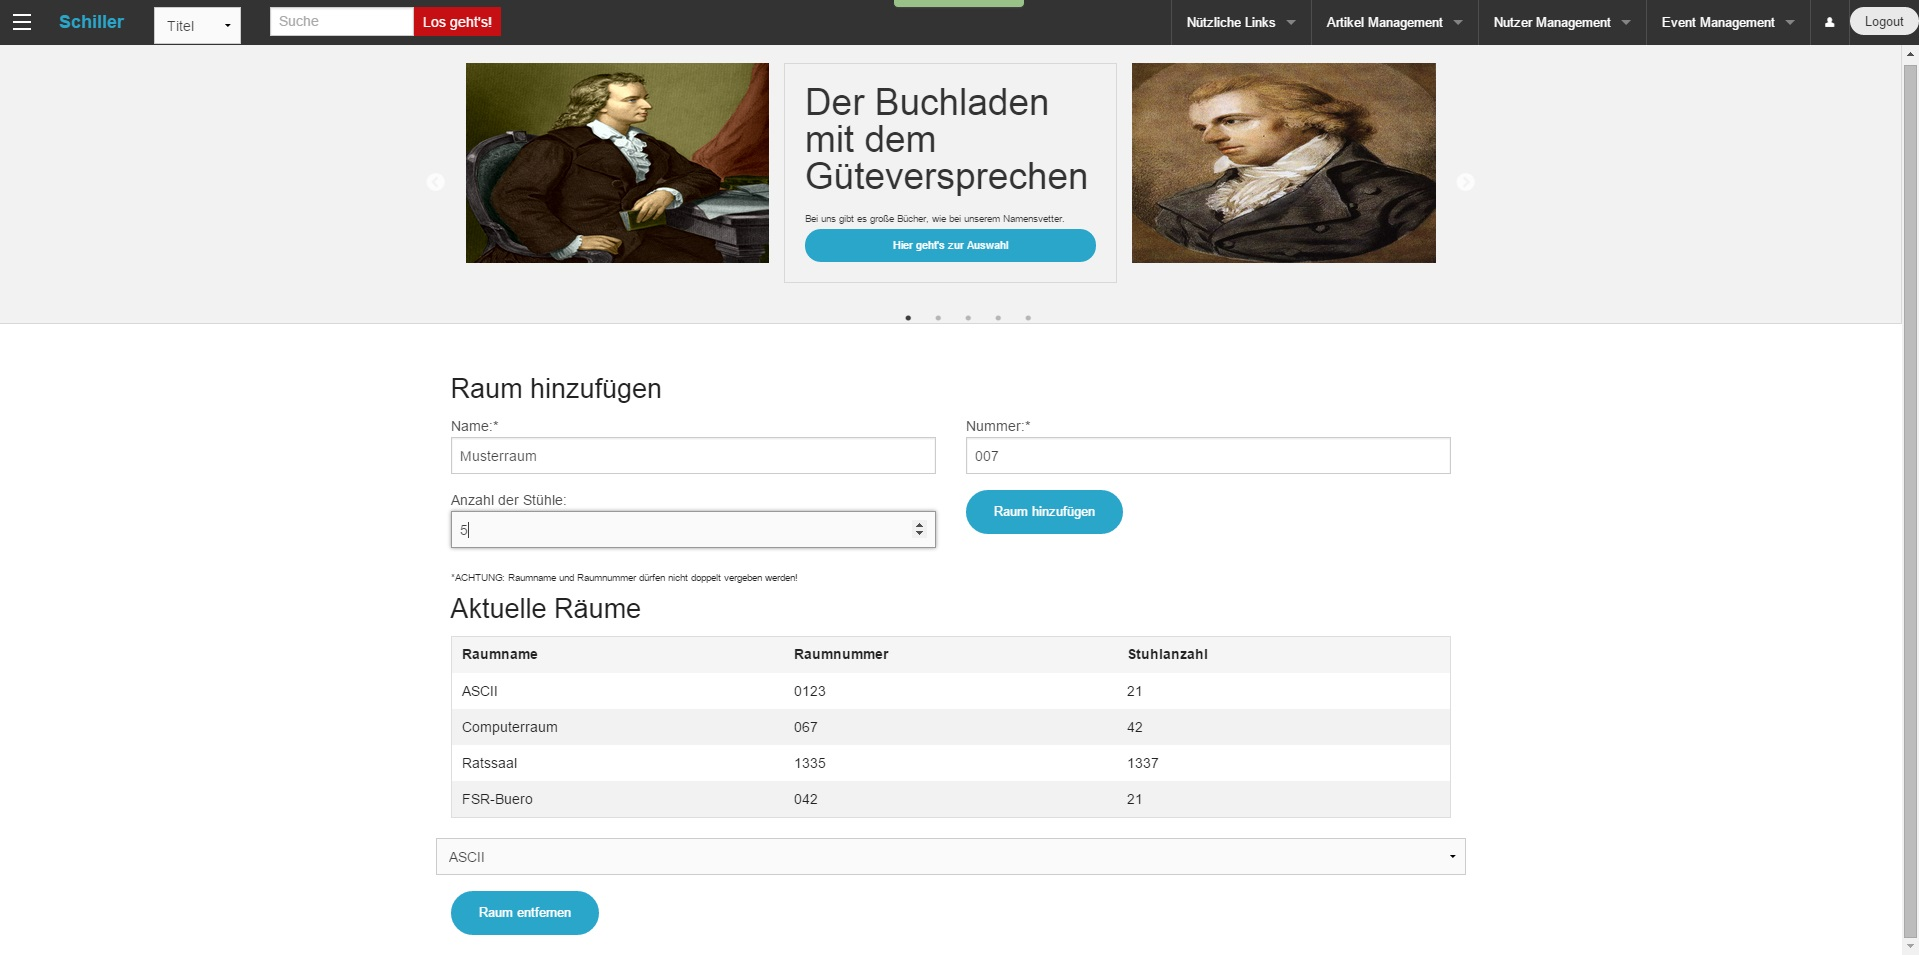
\includegraphics[width=1.0\textwidth]{Raeume.jpg}
\caption{Raumbearbeitung}
\end{figure}
\smallskip

\FloatBarrier

\end{document}